\documentclass{../lab}

\labacronym{NMR}
\labtitle{Nuclear Magnetic Resonance}

%\newcommand{\PulsedNMR}{http://experimentationlab.berkeley.edu/PulsedNMR}
%\newcommand{\Physics111LibrarySite}{http://physics111.lib.berkeley.edu/Physics111/Reprints/NMR/NMR_index.html}

\begin{document}

\maketitle

\tableofcontents

\section{Nuclear Magnetic Resonance CW and Pulsed Description (NMR)}

\begin{enumerate}
    \item \textbf{Note that there is NO eating or drinking in the 111-Lab anywhere, except in rooms 282 \& 286 LeConte on the bench with the BLUE stripe around it.} Thank You the Staff.
\end{enumerate}

In 1945 Felix Bloch (Stanford) and Edward Purcell (Harvard) discovered nuclear magnetic resonance in ordinary matter, for which they were awarded the Nobel Prize in 1952. This phenomenon has found many applications in science and technology, including magnetic resonance imaging used in medical practice.

In the NMR experiment, nuclear dipoles (the samples) are placed in a static magnetic field of about 3800 Gauss, and in a time-varying radio-frequency magnetic field perpendicular to the static field. The static field causes Zeeman-effect splitting between sub-states, and the radio-frequency field is tuned to the Larmor frequency so that it induces transitions between the sub-states. The resonance condition is observed using the Bloch two-coil induction technique. You will observe the resonance of the proton and fluorine nucleus. You will learn techniques of lock-in detection and signal averaging.

The second part of this experiment uses a pulsed radio-frequency field rather than a continuous-wave (CW) field. Signals are detected immediately after the pulsed excitation stops. The observable effects are similar to the free vibration or ringing of a resonant cavity on the atomic scale. This is the basis of Magnetic Resonance Imaging in the medical field today.

\begin{enumerate}
    \item Pre-requisites: Physics 137B

    \item Days Allotted for the Experiment:

\end{enumerate}

\textbf{Click on words Pulsed NMR below for Pulsed NMR page:  }\href{http://experimentationlab.berkeley.edu/PulsedNMR}{\textbf{Pulsed NMR}}

Reprints and other information can be found on the \href{http://physics111.lib.berkeley.edu/Physics111/Reprints/NMR/NMR\_index.html}{\textbf{Physics 111 Library Site}}

This lab will be graded 30\% on theory, 40\% on technique, and 30\% on analysis. For more information, see the \href{\AdvancedLabSyllabus}{\textbf{Advanced Lab Syllabus}}.

Comments: E-mail \href{\MailDonOrlando}{\textbf{Don Orlando}}

\section{NMR Pictures}

\noindent
\href{http://experimentationlab.berkeley.edu/sites/default/files/images/NMR_Exp_3496.jpg}{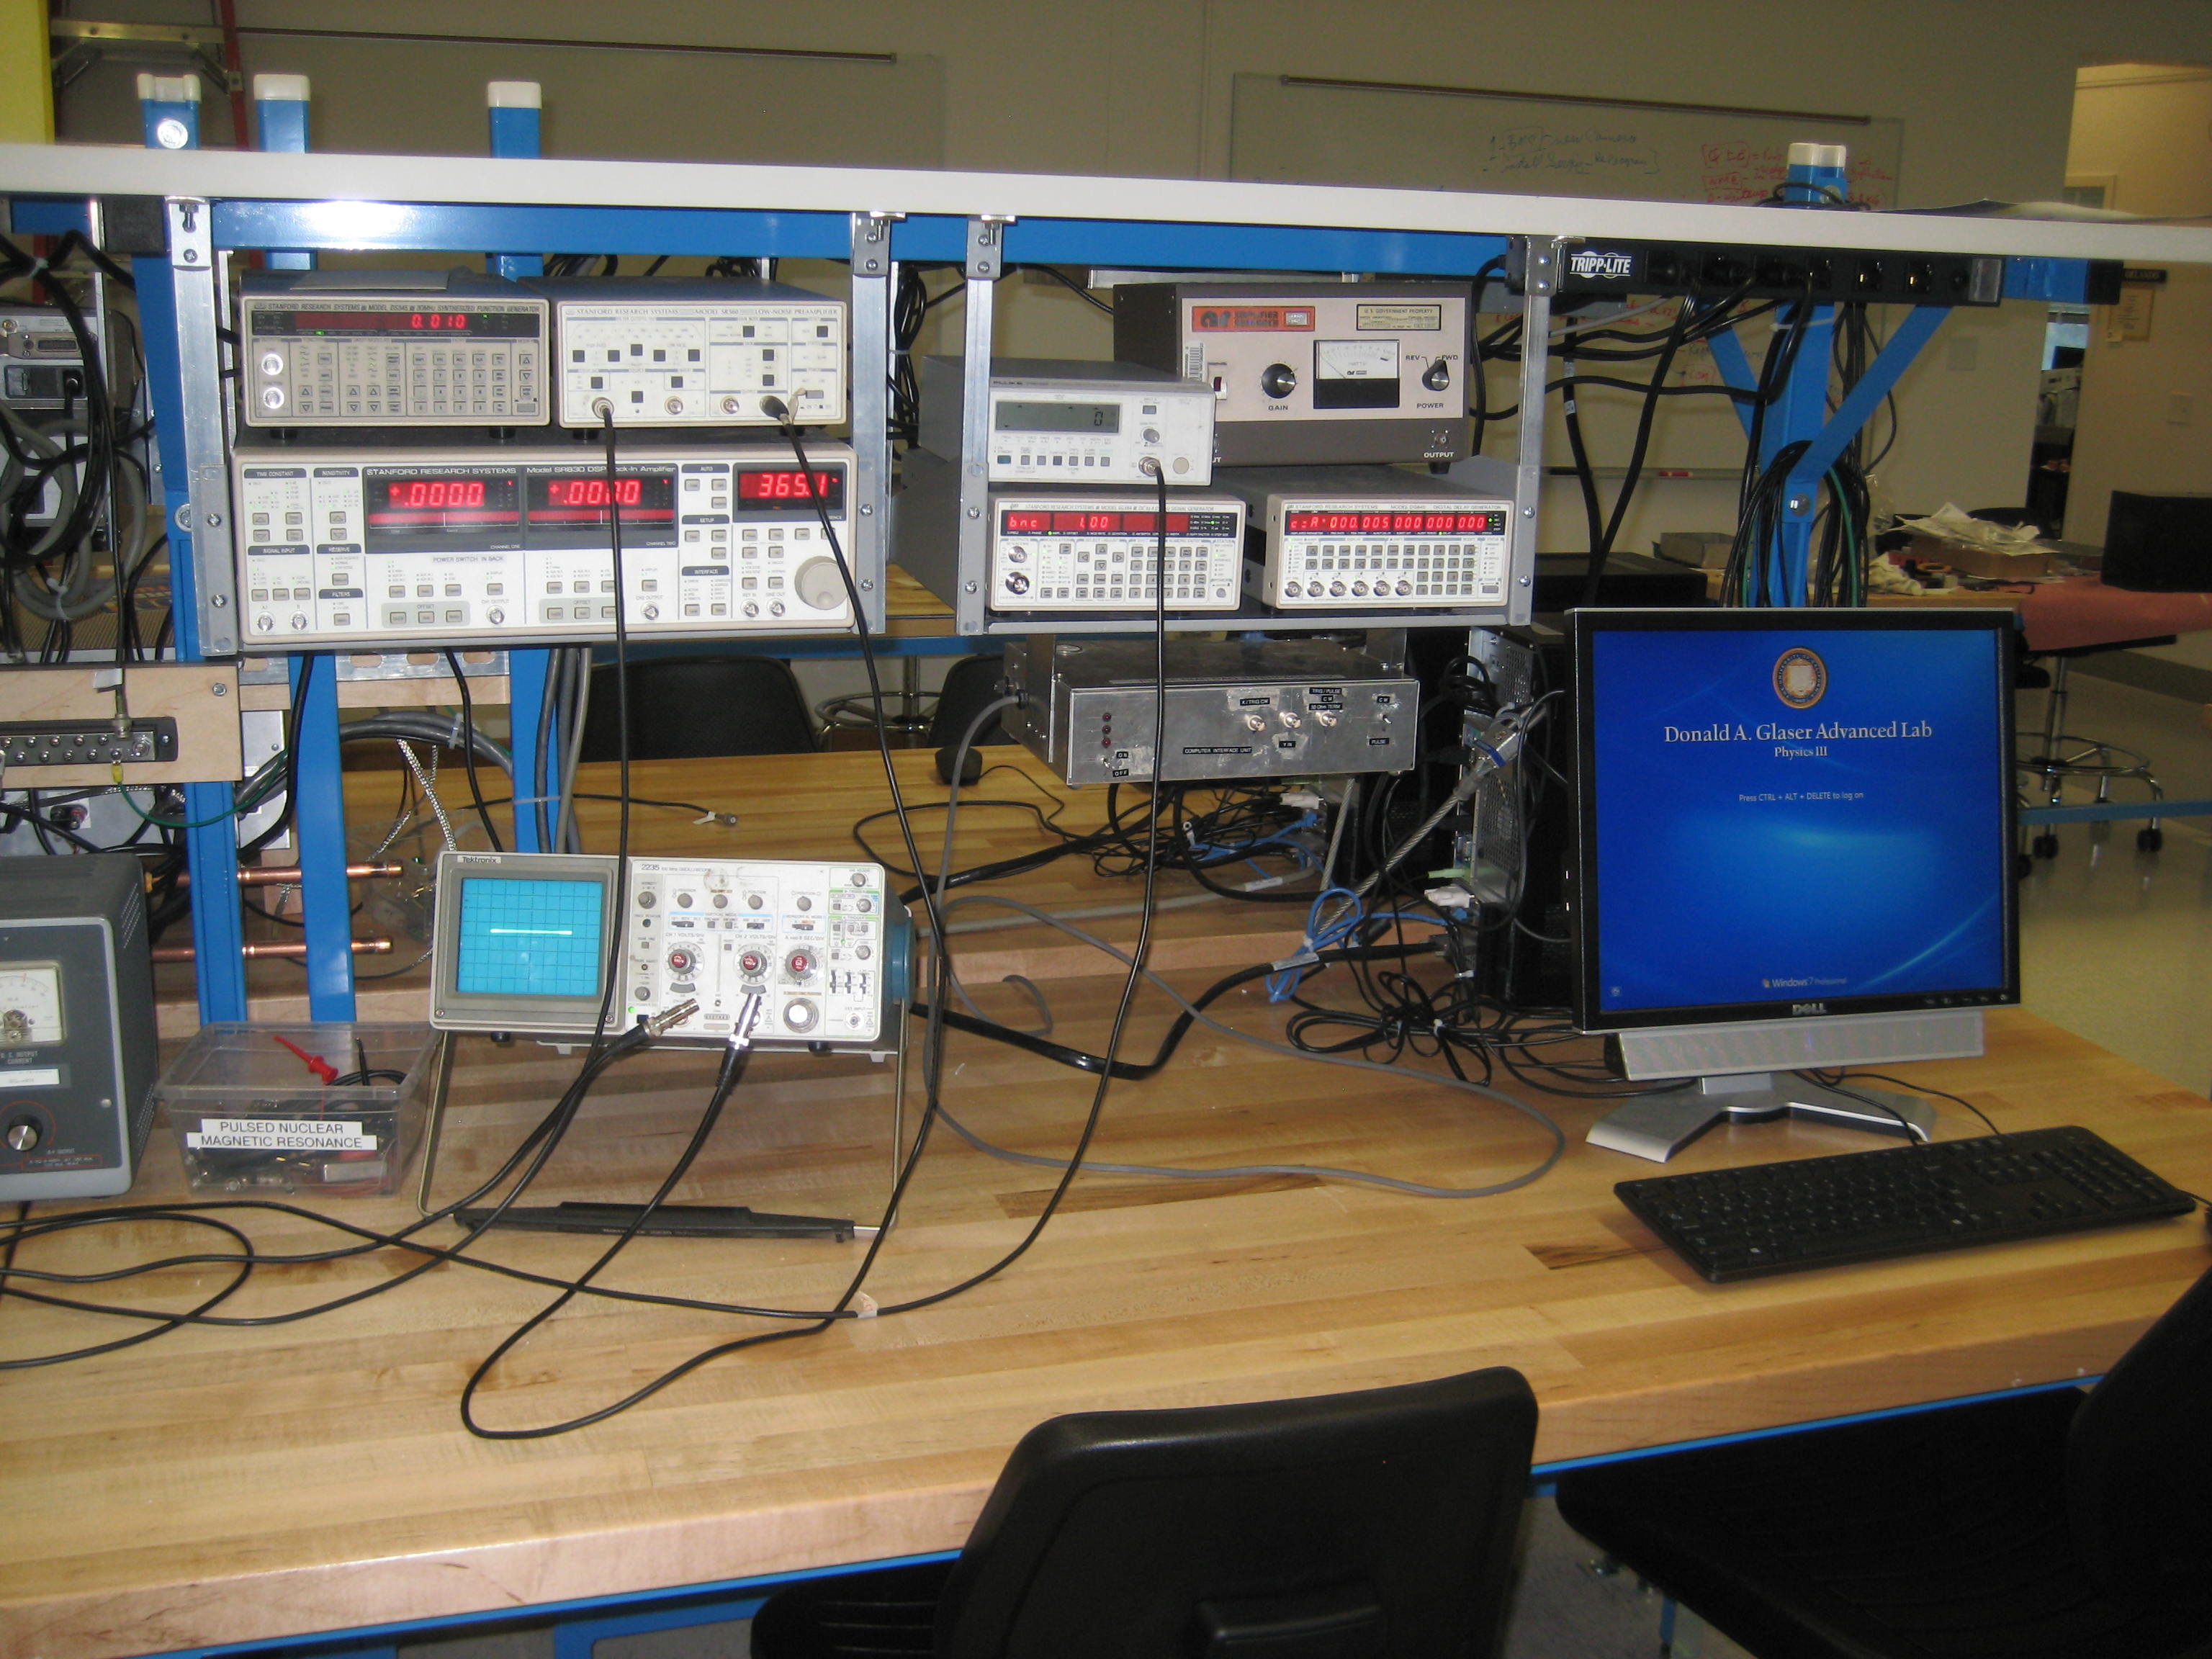
\includegraphics[width=0.33\linewidth,keepaspectratio]{images/NMR_Exp_3496.jpg}}
\href{http://experimentationlab.berkeley.edu/sites/default/files/images/NMR_Exp_3557.jpg}{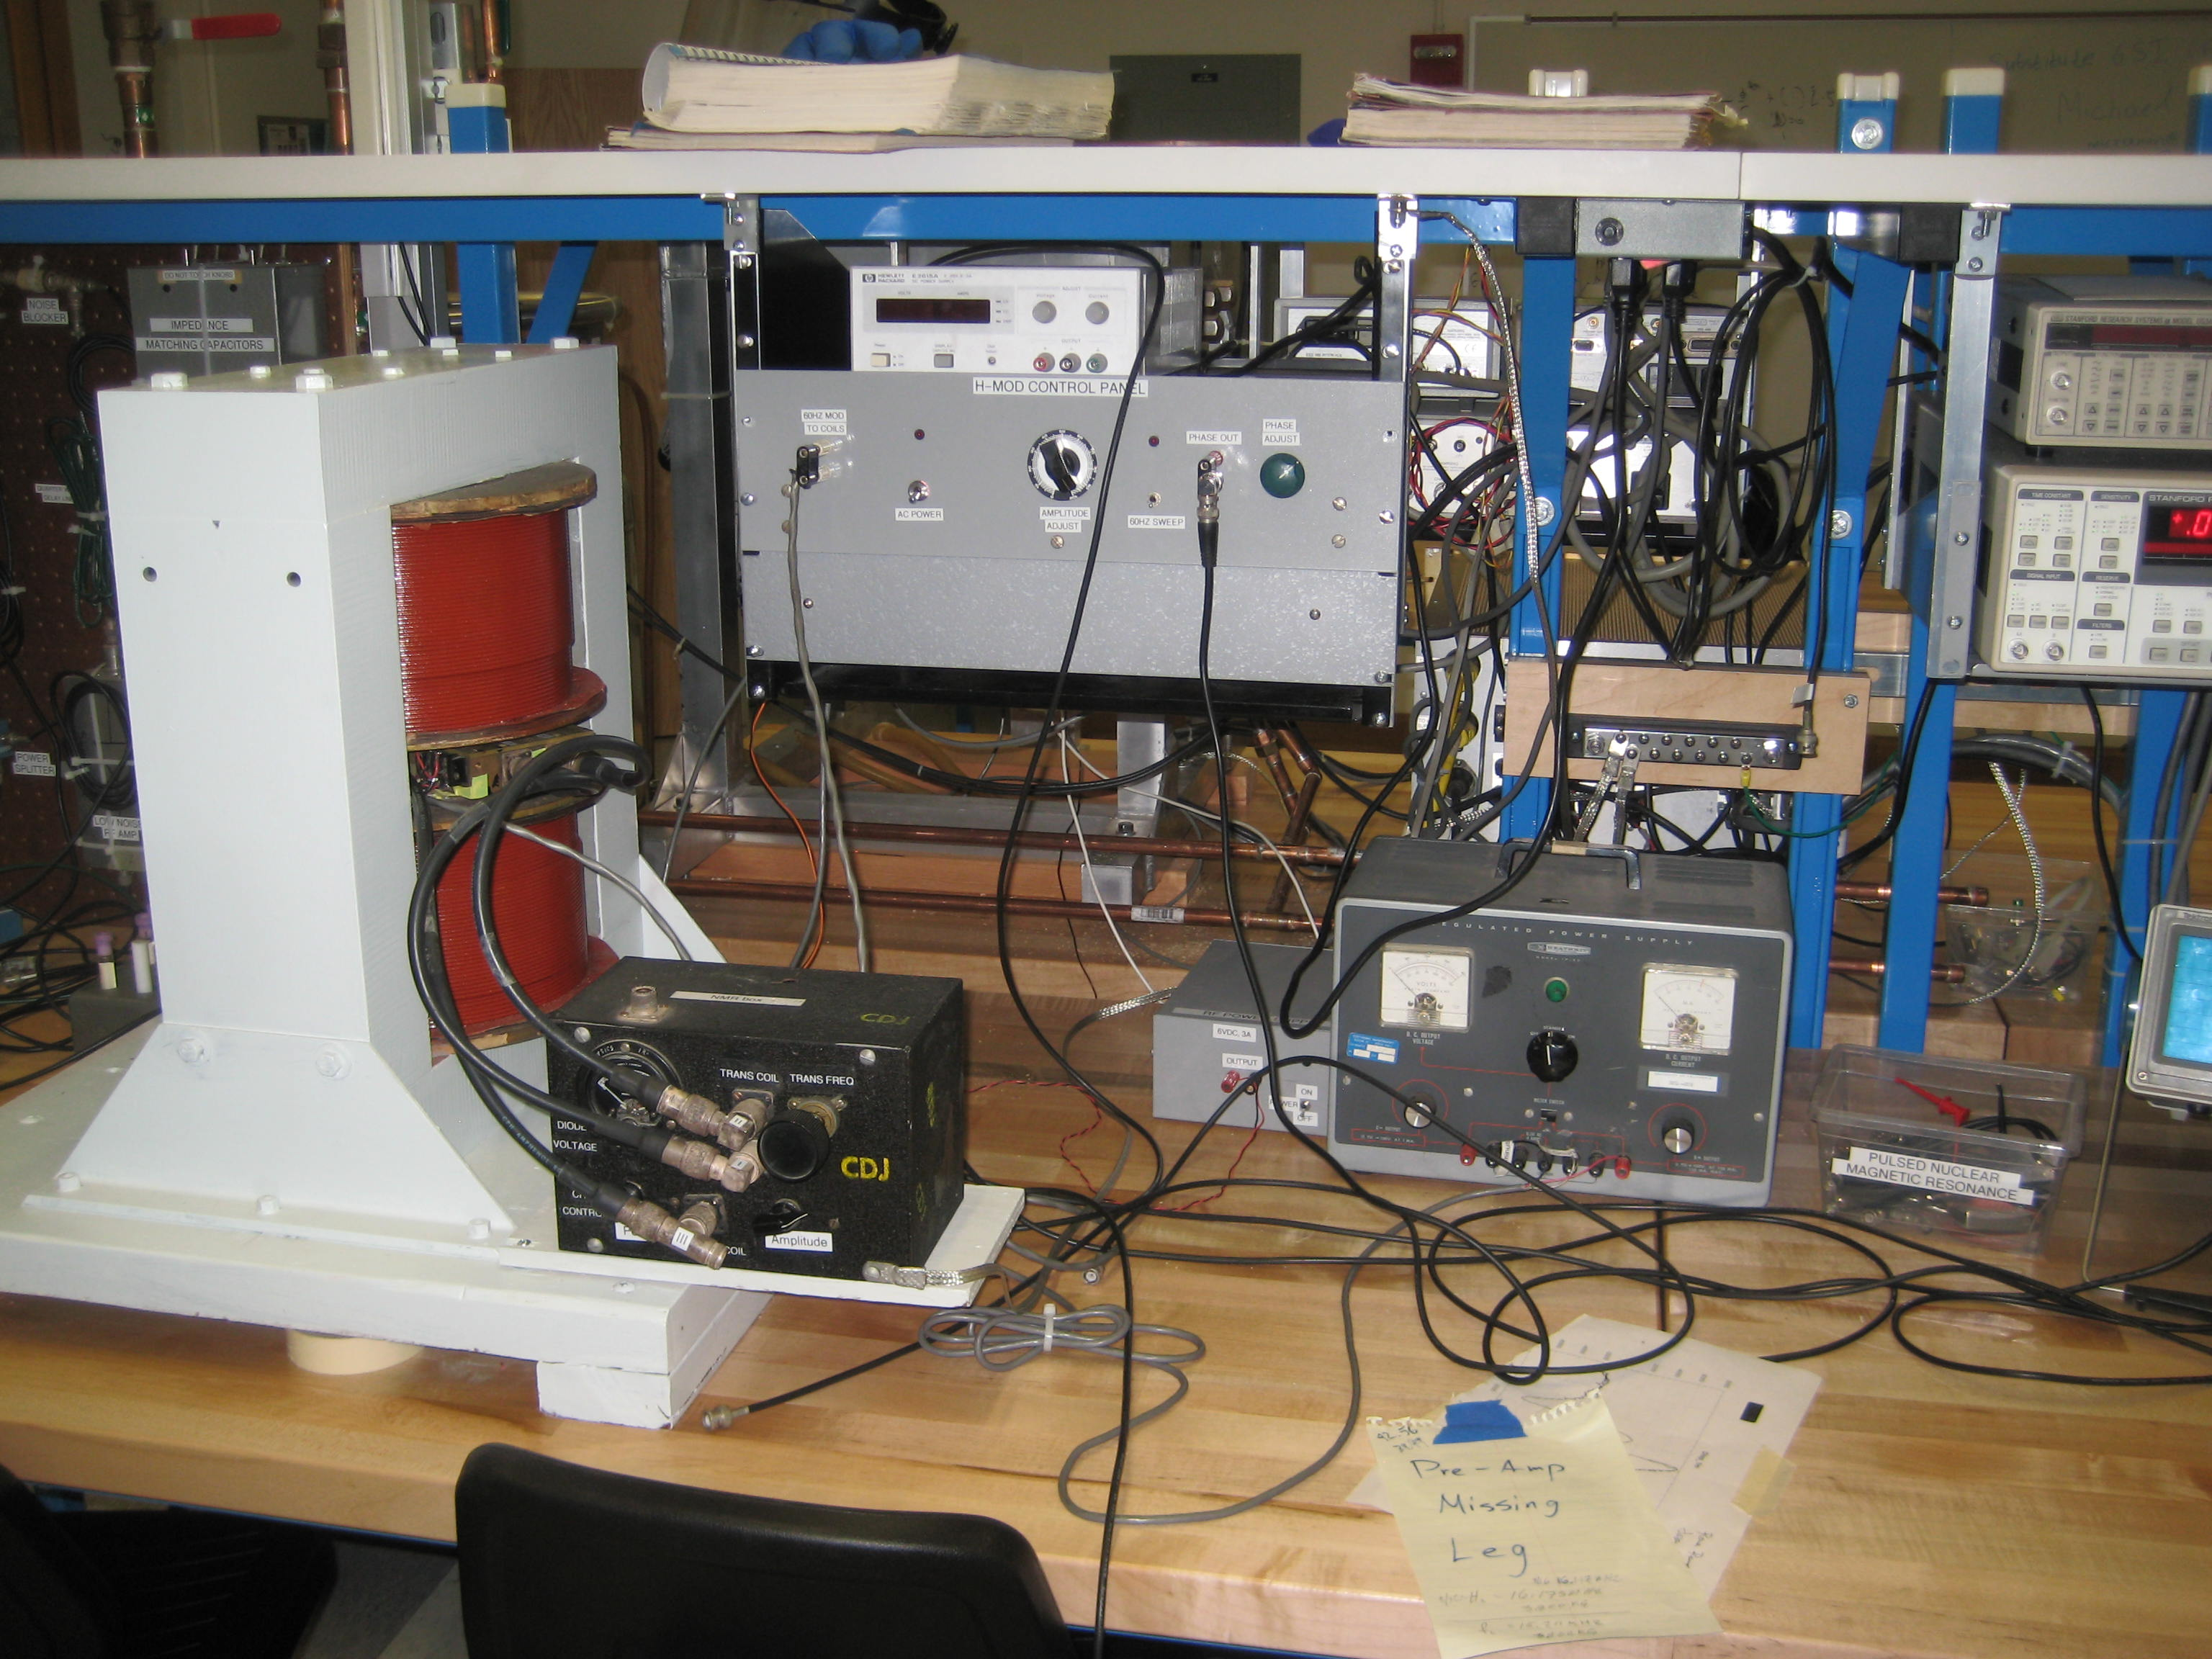
\includegraphics[width=0.33\linewidth,keepaspectratio]{images/NMR_Exp_3557.jpg}}
\href{http://experimentationlab.berkeley.edu/sites/default/files/images/NMR_Exp_3559.jpg}{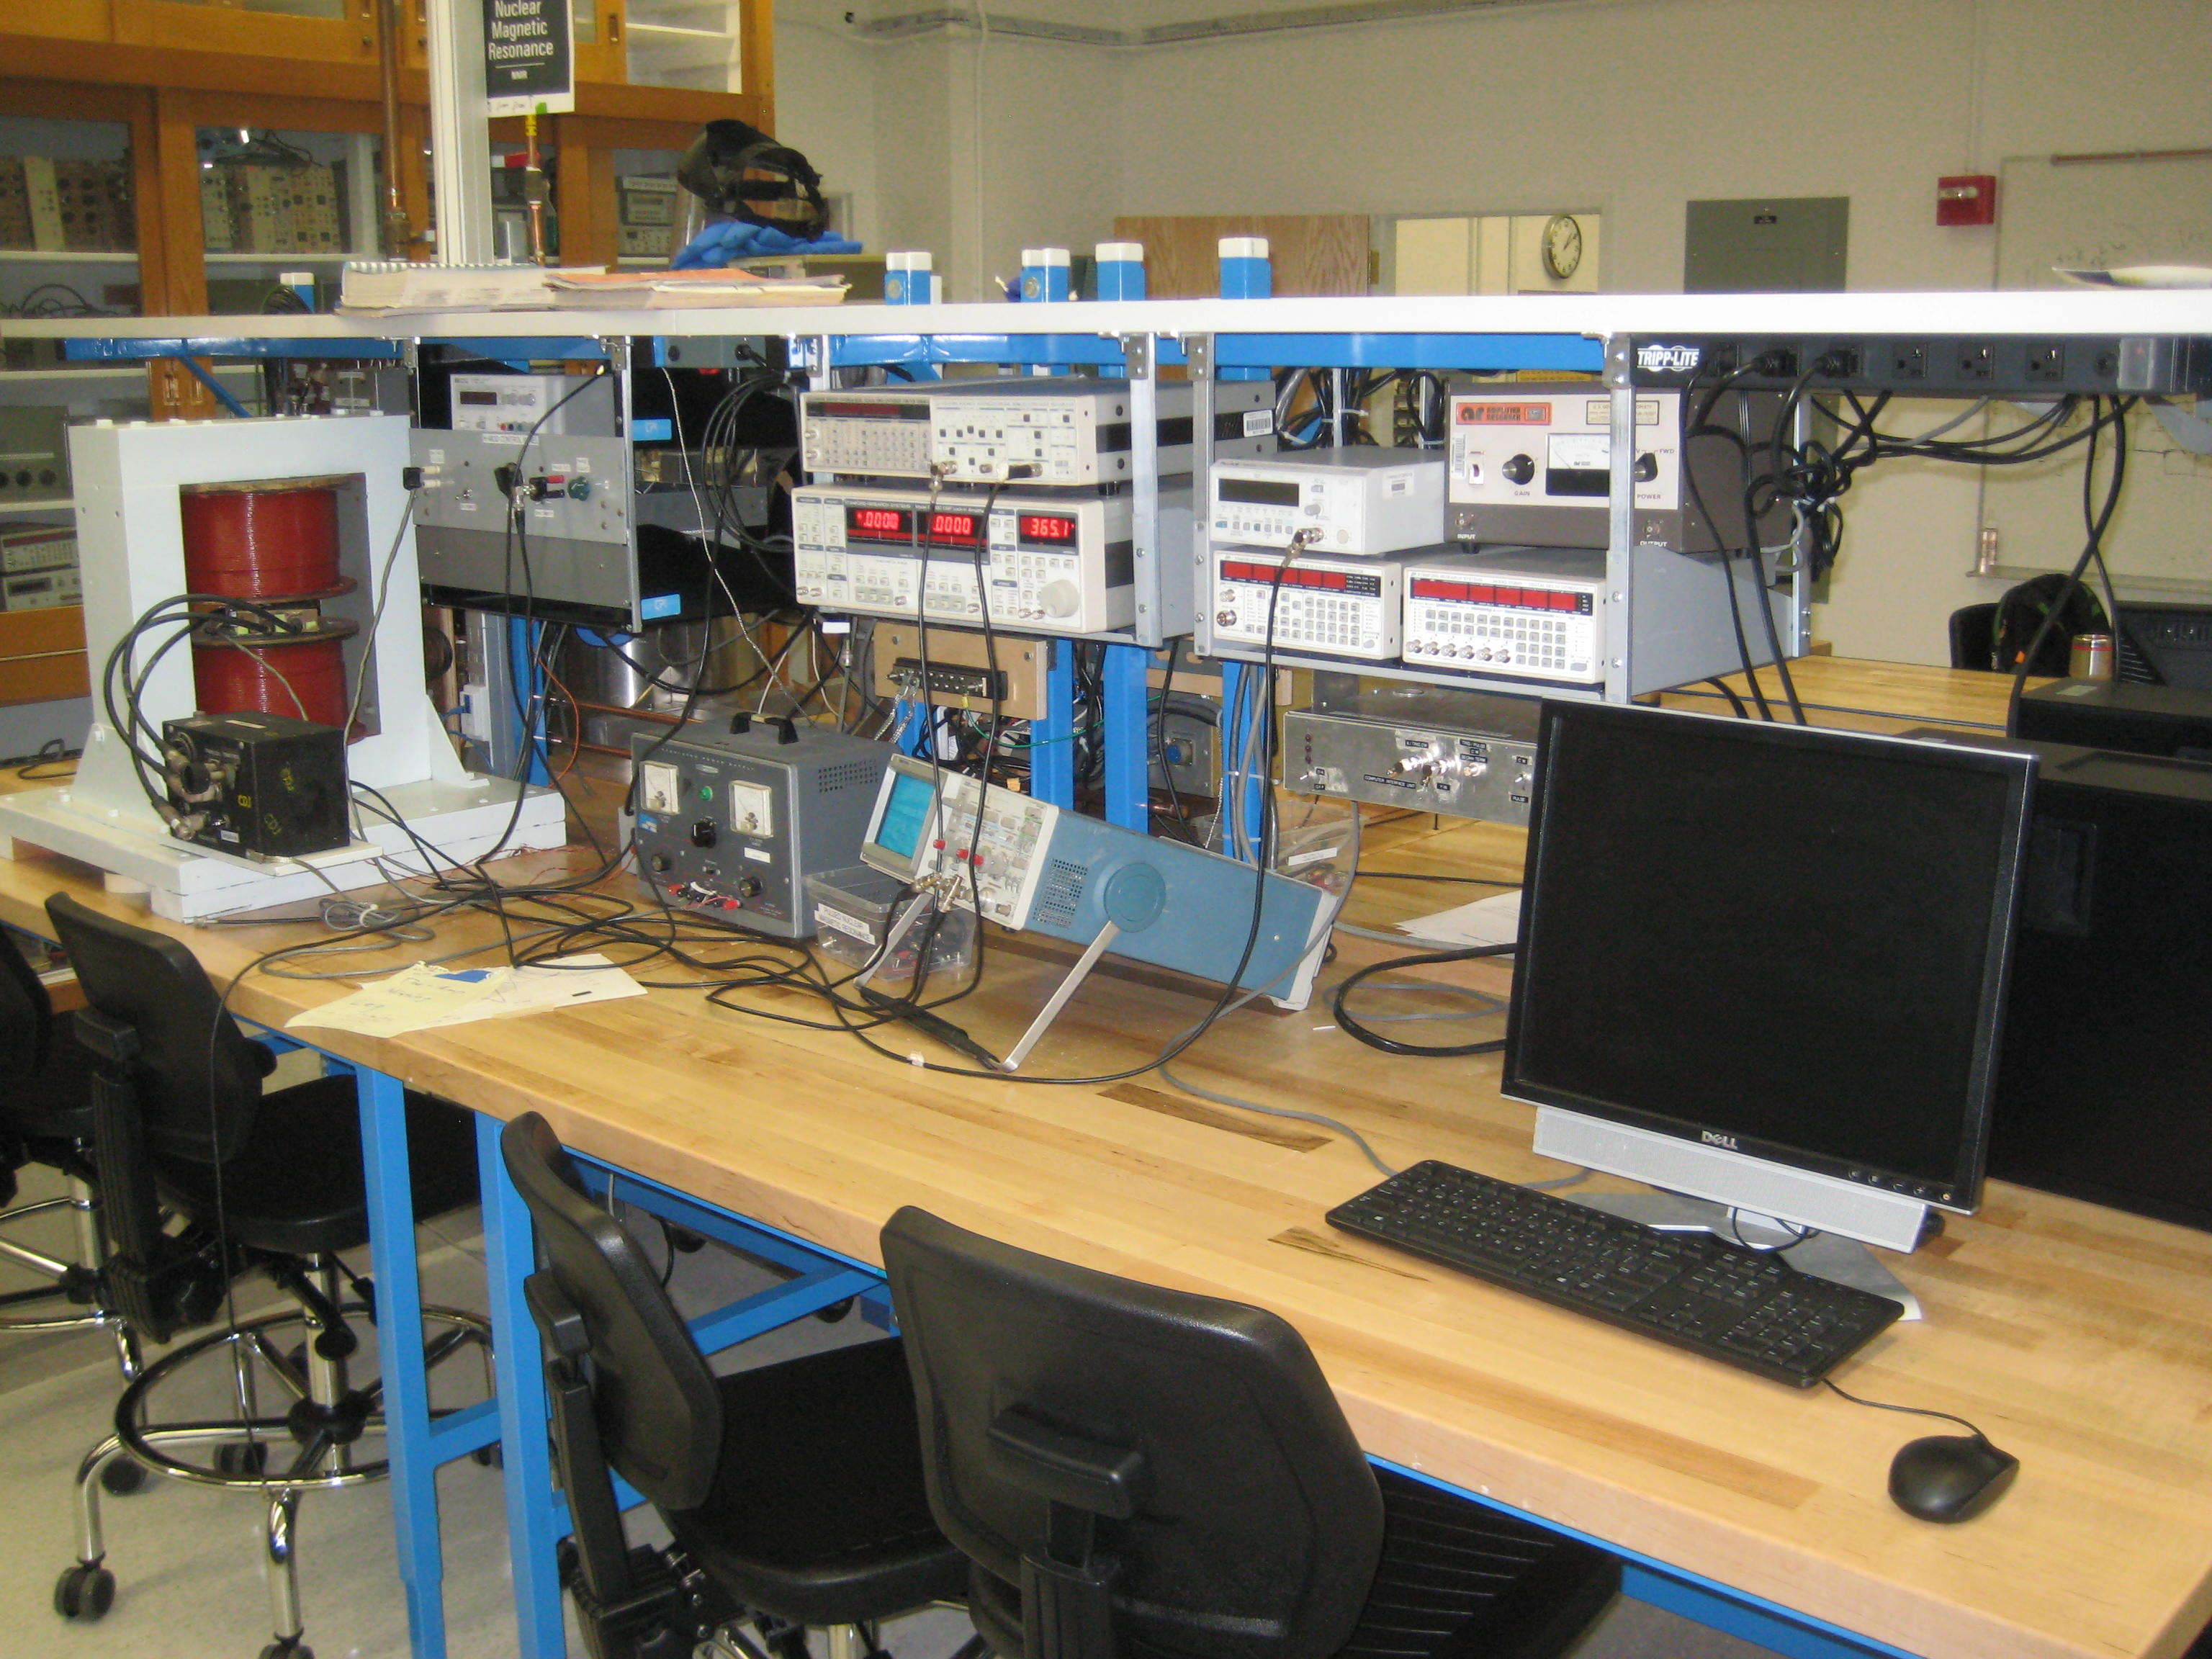
\includegraphics[width=0.33\linewidth,keepaspectratio]{images/NMR_Exp_3559.jpg}}
\href{http://experimentationlab.berkeley.edu/sites/default/files/images/NMR_Head-in-Magnet_3560.jpg}{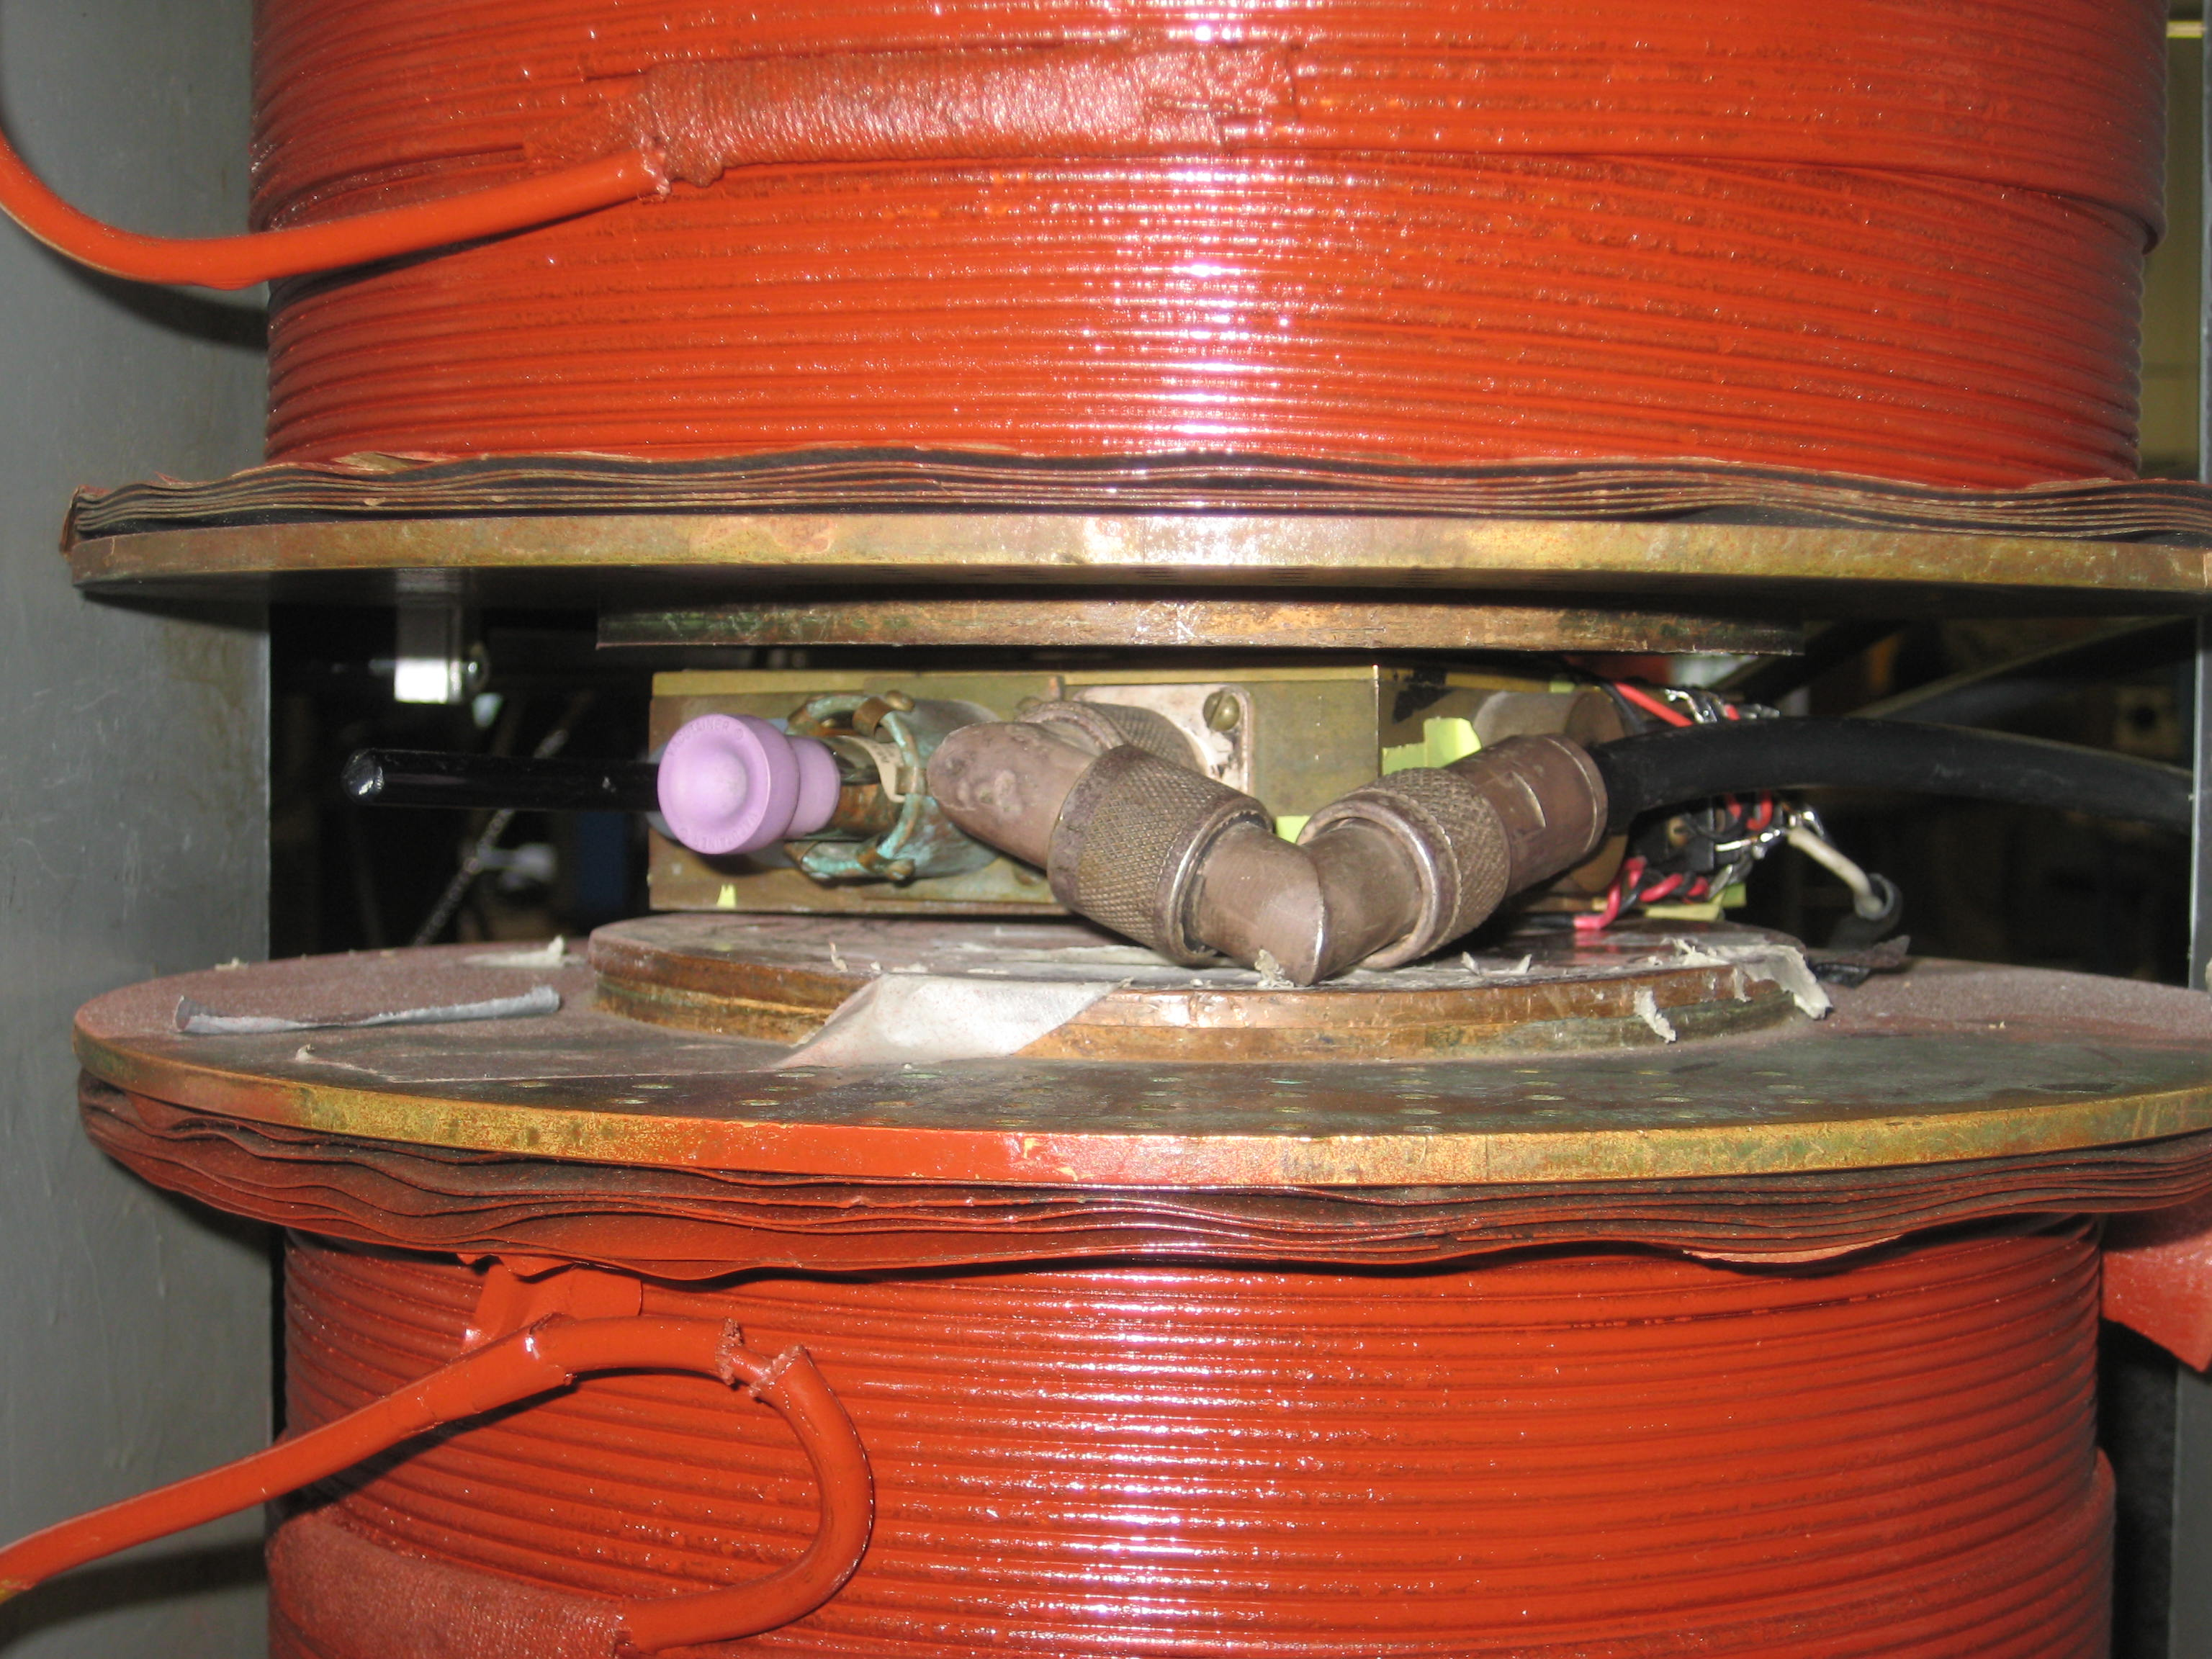
\includegraphics[width=0.33\linewidth,keepaspectratio]{images/NMR_Head-in-Magnet_3560.jpg}}
\href{http://experimentationlab.berkeley.edu/sites/default/files/images/PNMR_3494.jpg}{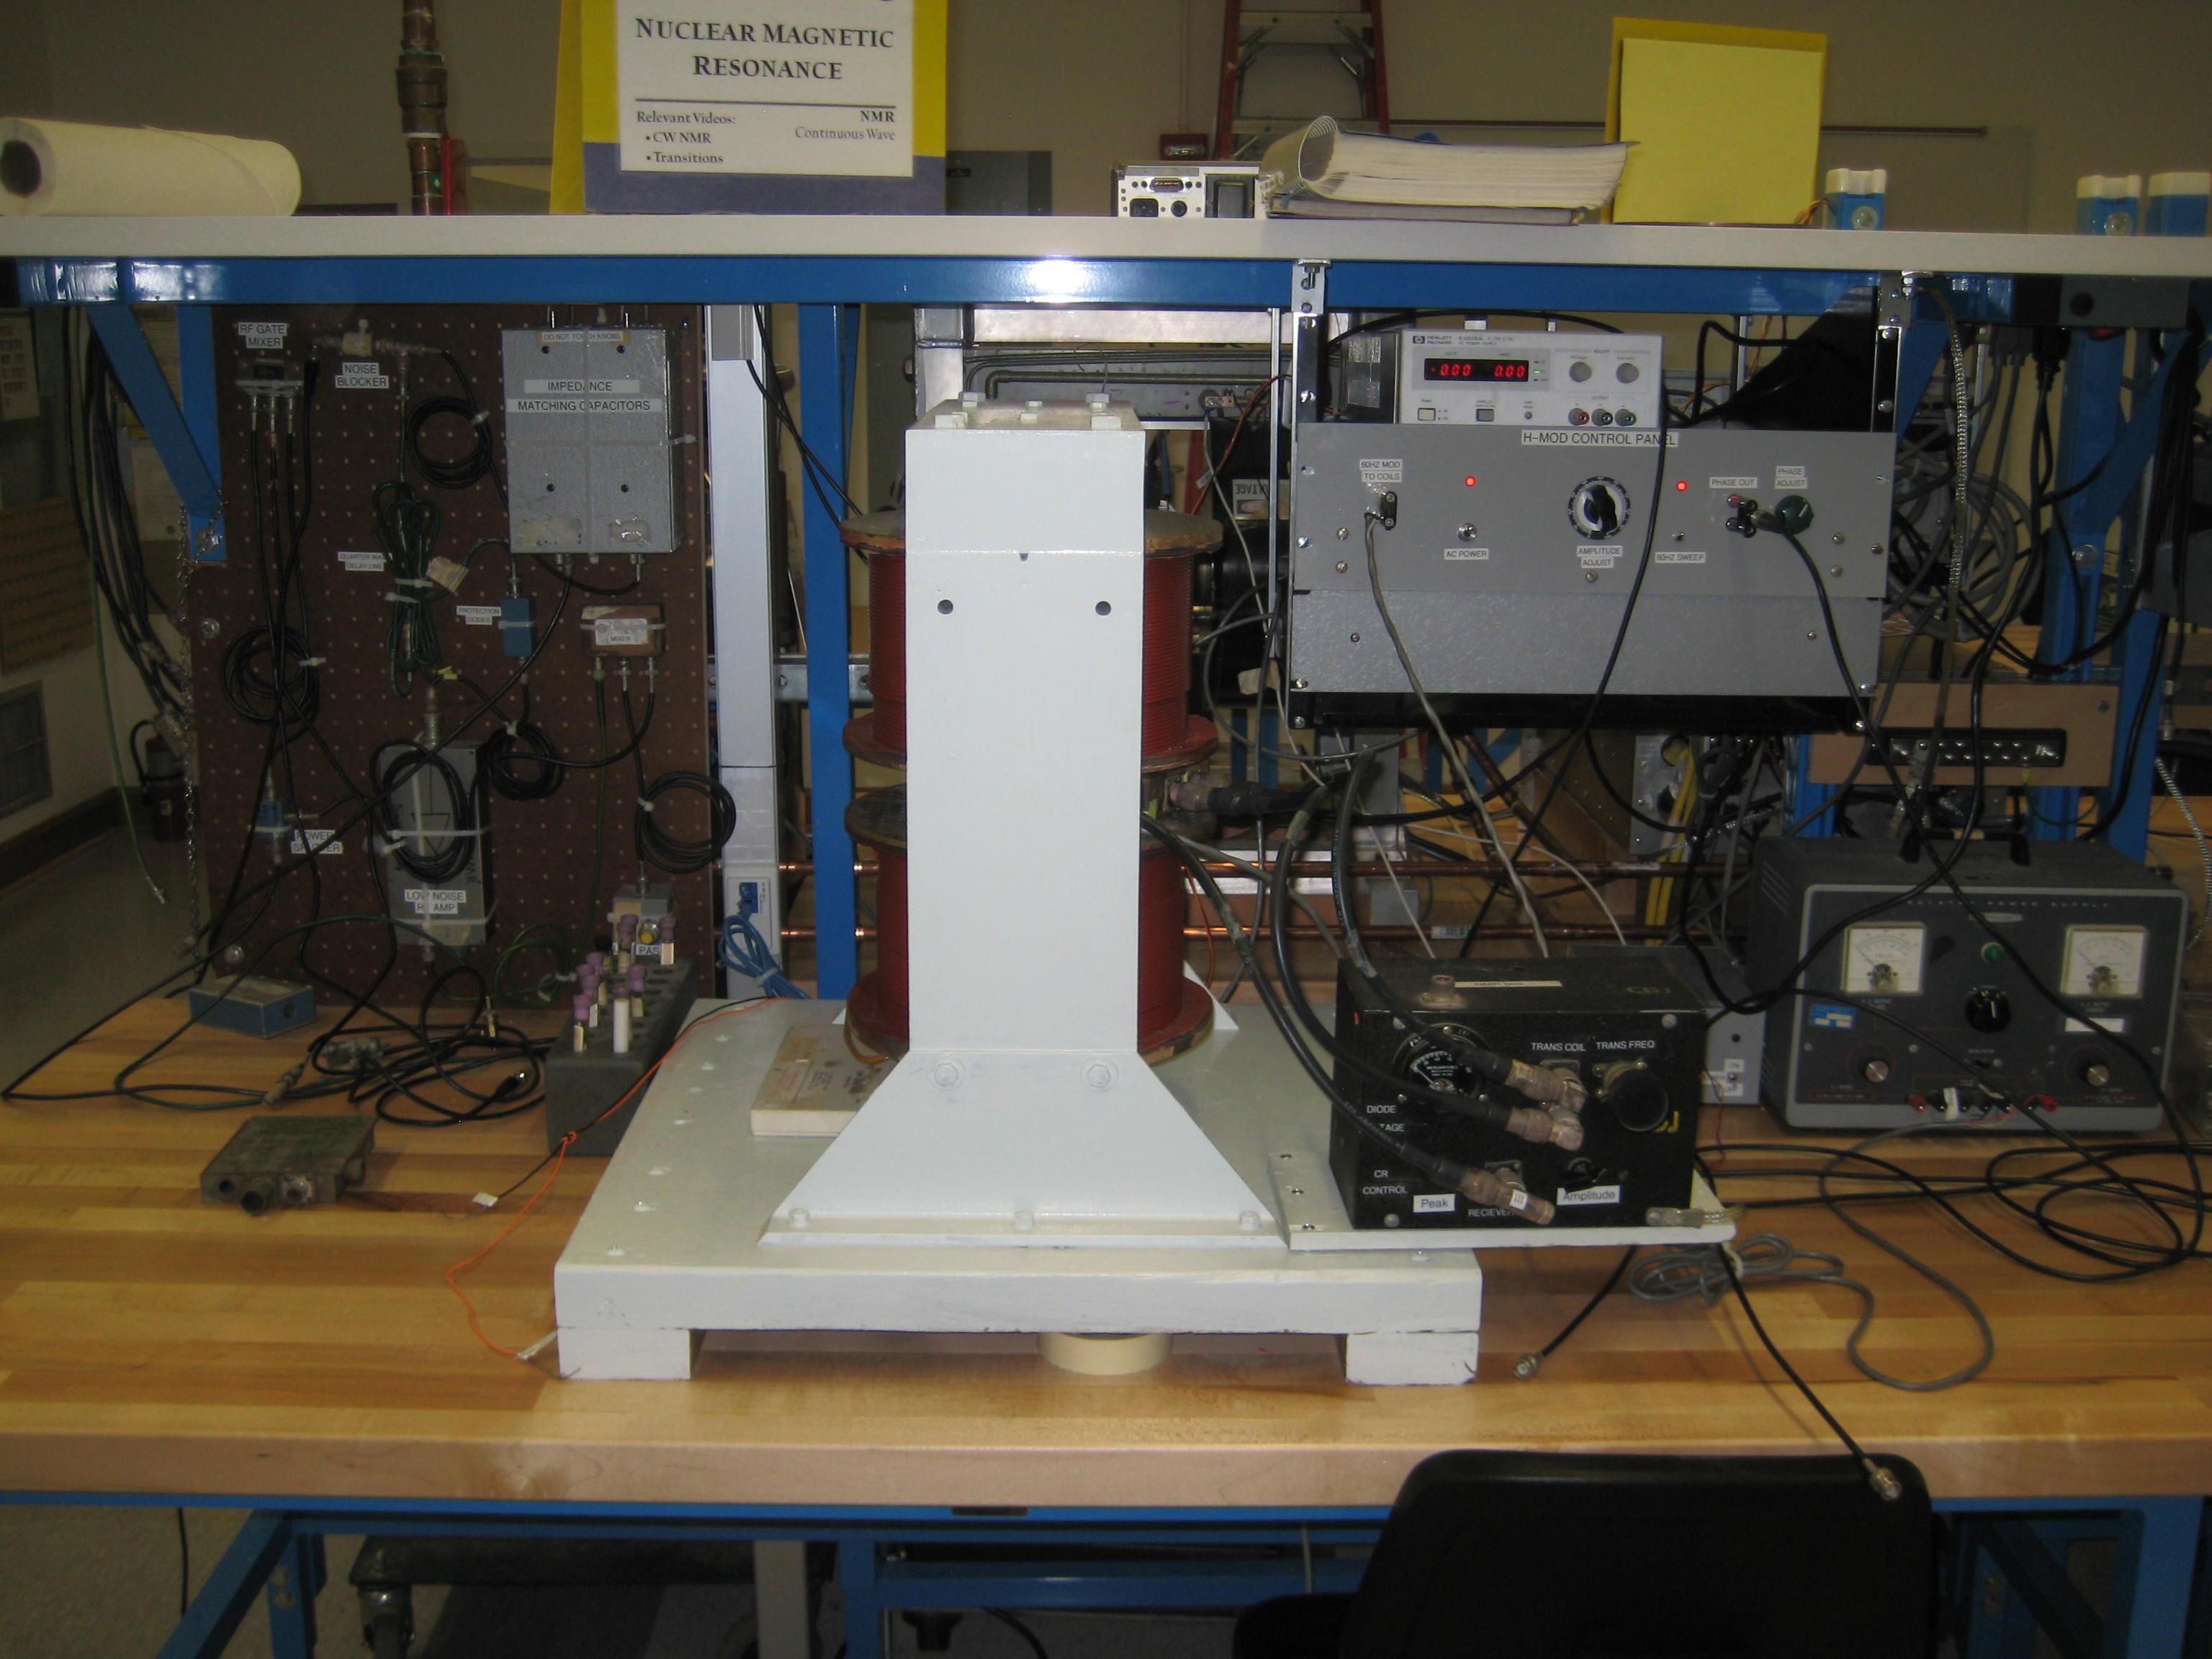
\includegraphics[width=0.33\linewidth,keepaspectratio]{images/PNMR_3494.jpg}}
\href{http://experimentationlab.berkeley.edu/sites/default/files/images/PNMR_3495.jpg}{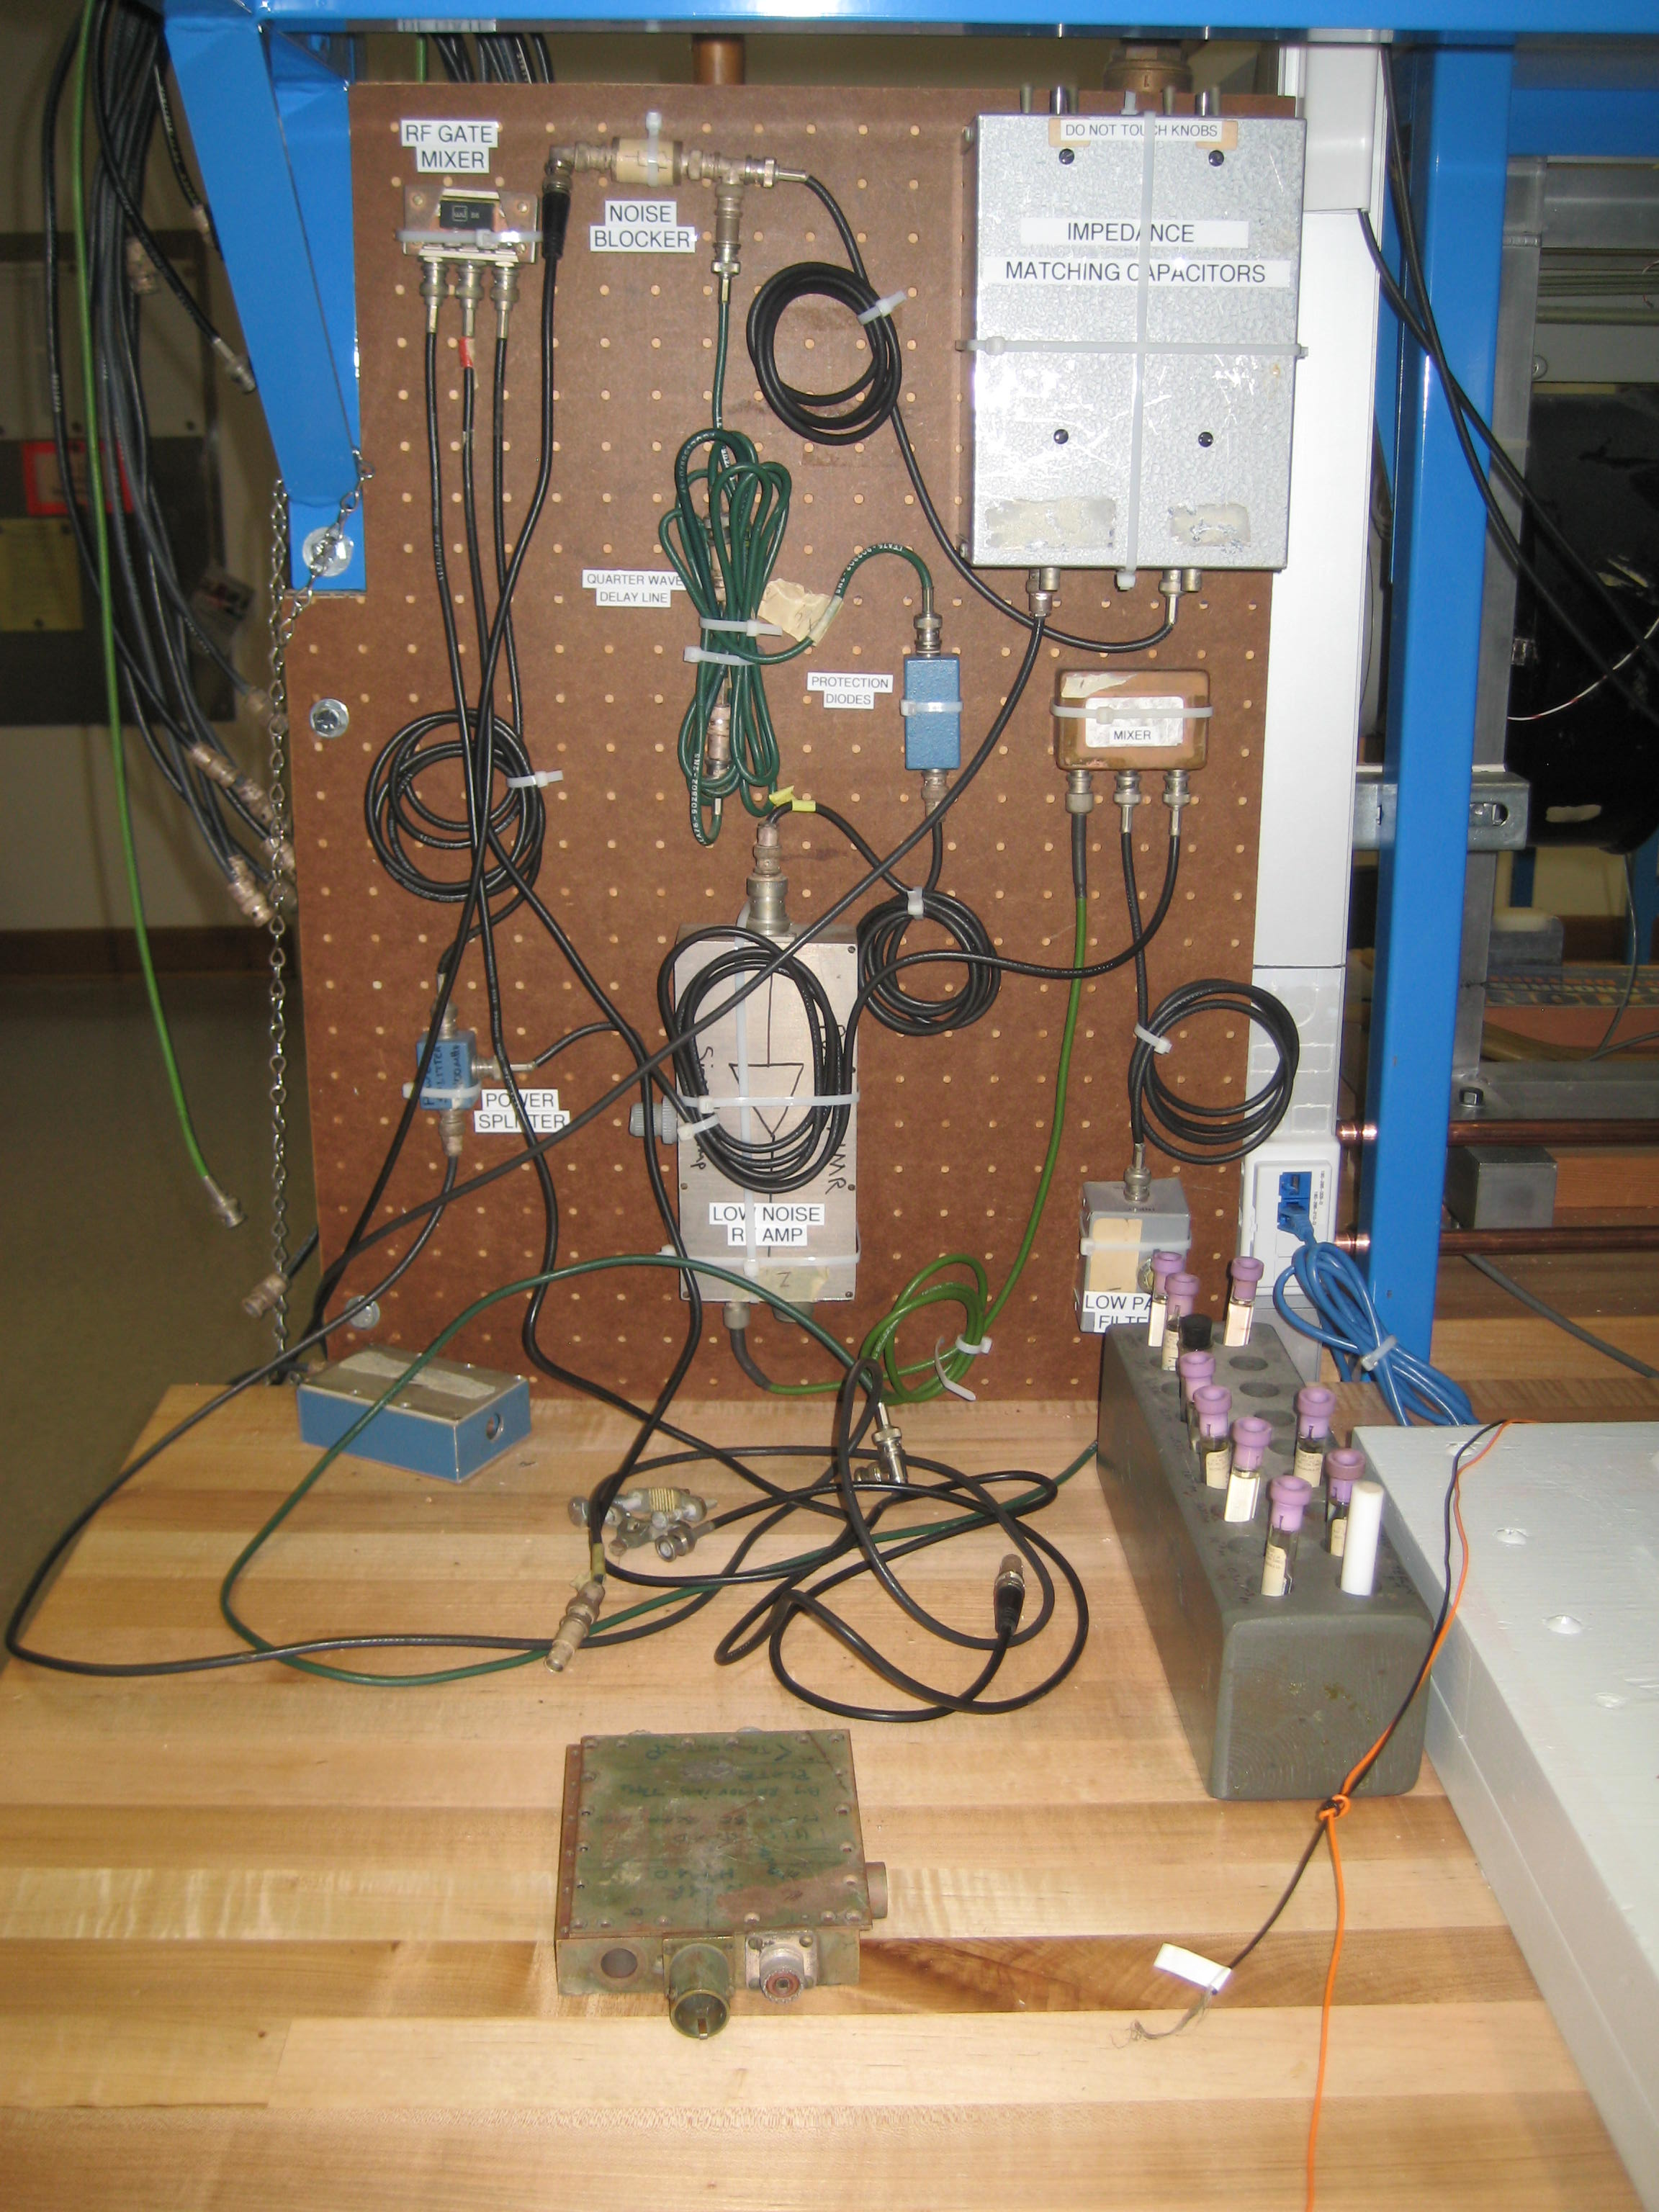
\includegraphics[width=0.33\linewidth,keepaspectratio]{images/PNMR_3495.jpg}}

\section{Before the 1st Day of Lab}

\textbf{Complete the following before your experiment's scheduled start date}

\begin{enumerate}
    \item View the two videos \href{http://youtu.be/q\_Rtbr7YEJY}{\textbf{CW NMR}} and \href{http://youtu.be/\_sXDn-ChOUY}{\textbf{Pulsed NMR}}.

    \item Complete the \href{http://experimentationlab.berkeley.edu/NMRPreLab}{\textbf{NMR Pre Lab and Evaluation}} sheets. Print, fill out the answers, and turn in with your report. The Pre-Lab must be printed separately. Discuss the experiment and pre-lab questions and answers with any faculty member or GSI and get it signed off by that faculty member or GSI. Turn in the signed pre-lab sheet with your lab report.

    \item View the Transitions Lecture, \href{http://youtu.be/xOMgdVP3AfE}{\textbf{Transitions}}

    \item \emph{Check points are examination points that are placed in this lab where you must STOP and call a GSI or professor to make sure you understand what's expected. There could  be multiple check points throughout your lab so make sure you don't skip them since there is a \href{http://experimentationlab.berkeley.edu/nmrcheckpoints}{\textbf{sign off sheet}} that must be turned in with your lab report.}

    \item Last day of the experiment please fill out the \href{\ExperimentEvaluation}{\textbf{Experiment Evaluation}}

\end{enumerate}

\textbf{Suggested Reading:}

\begin{enumerate}
    \item Bloch, Felix ``\href{http://physics111.lib.berkeley.edu/Physics111/Reprints/NMR/02-Nuclear\_Magnetism.pdf}{\textbf{Nuclear Magnetism}}''; American Scientists: \textbf{43}, 48-62 (Jan 1955).

    \item C. Kittel, \emph{Introduction to Solid State Physics}, 5th ed., John Wiley (1976). Read pp. 479-509 for a brief-quantitative expose of the main ideas. Located in the Physics and Astronomy Library \#QC176.K51

    \item L Yuan and C. S. Wu, \emph{\href{http://physics111.lib.berkeley.edu/Physics111/Reprints/NMR/01-Methods\_of\_Experimental\_Physics.pdf}{\textbf{Methods of Experimental Physics}}}, Part B, Vol. 5, Academic Press (1963), pp. 104-123 (Section 2.4.1.4). This reference discusses all the ideas necessary to do the experiment, which uses the two-coil Bloch method.

    \item F. Bloch, ``\href{http://prola.aps.org/abstract/PR/v70/i7-8/p460\_1}{\textbf{Nuclear Induction}}'', \emph{Physical Review \textbf{70}, 460 (1946). Bloch's two-coil method is used in this experiment. }

    \item R. Schumaker and W. A. Benjamin, \emph{Introduction to Magnetic Resonance}, 1970. Read Ch. 2 and Ch. 3. Located in the Physics and Astronomy Library \#QC762.S34
\end{enumerate}

More \hyperref[References]{References}

You should keep a laboratory notebook. The notebook should contain a detailed record of everything that was done and how/why it was done, as well as all of the data and analysis, also with plenty of how/why entries. This will aid you when you write your report.

\section{Objectives}

\begin{itemize}
    \item Learn what real experimental physics is about

    \item Learn the synergy between experimental and theoretical work

    \item Learn to use pieces of equipment that are commonly used in research

    \item Learn how measurements are performed, analyzed, and interpreted.

    \item Learn how to present your work and results

    \item Learn problem solving strategies

    \item Learn how to manage and organize your time

\end{itemize}

\section{Introduction}

In 1952, Felix Bloch and Edward Purcell received the Nobel Prize in physics for their discovery of nuclear magnetic resonance in 1945. Bloch's method of observation is now widely used in many areas of science and technology. NMR is a sensitive probe for determining the local magnetic field at the location of the nuclei in matter. It gives us information about nuclear spins and their surroundings. In the medical field, it is called Magnetic Resonance Imaging to avoid the use of the word ``nuclear''. This experiment has the following objectives:

\begin{enumerate}
    \item To observe the phenomena of nuclear magnetic resonance (NMR) of protons in H2O and other liquids

    \item To observe the absorption and dispersion line shapes of NMR under slow passage and under non-adiabatic passage conditions, and to study their dependence on the concentration of paramagnetic ions added to the liquid

    \item To measure the ratio of the magnetic moment of F19 to that of the proton

    \item To use the technique of lock-in detection to get improved signal-to-noise ratios in the NMR detection.

\end{enumerate}

A former student commented, ``The best thing that can be said about NMR is that, in beginning of the experiment, a student feels overwhelmed by its complexity. As you become more familiar with it, this feeling is replaced by curiosity and eventually understanding.'' This is to say that while there is a great deal to learn initially about NMR, given time and a lot of effort the pieces do fall into place, and the result is an unusually rewarding experiment.

\section{Theory}

Conceptually this experiment is quite simple, but how the data are recorded is not. It helps to know what we are going to do before we discuss what pieces of equipment we use.

Suppose we place a single nucleus between the south and north poles of the magnet. The interaction between the magnetic moment of the nucleus with the local magnetic field creates equal and opposite forces that form a torque upon the nucleus in the classical picture. The magnetic moment then begins to rotate about the vertical axis. This rotation is called Larmor ``precession''. The frequency of this precession is called the Larmor frequency. In this experiment we will place the sample of protons in a permanent magnet. This will force the protons to precess at the Larmor frequency and induce an electric field in a receiver coil that is wrapped around the sample. At the same time we will apply a radio frequency to the sample. This frequency will be tuned to the precession frequency, yielding a resonance. Our goal is to observe the nuclear magnetic resonance of the protons in the sample.

\begin{figure}[h]
    \centering
    \href{http://experimentationlab.berkeley.edu/sites/default/files/images/NMR1.jpg}{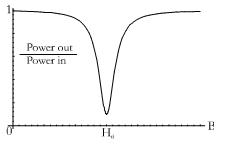
\includegraphics[width=0.3\linewidth]{images/NMR1.jpg}}
    \caption{Absorption signal of a magnetic resonance system as a function of the applied magnetic field.}
    \label{fig:AbsorptionSignal}
\end{figure}

In the quantum mechanical picture, a sample of protons in a magnetic field of strength $H_0$ has energy levels that are populated according to the Boltzmann distribution. When we send in photons (electromagnetic radiation) of energy $E = h\nu_0 = \hbar \gamma H_0$ the system absorbs some of the photons. This frequency, $\nu_0 = \gamma H_0 / 2\pi$ known as the Larmor frequency, is the resonance frequency of the system. At the resonance, the gyromagnetic ratio $\gamma $ can be determined from the ratio $2 \pi \nu_0 / H_0$. Alternatively, once we find the resonance frequency, we can determine $H_0$ using the known value of $\gamma$.

A typical resonance curve is shown in Figure~\ref{fig:AbsorptionSignal}. How shall we produce this curve so that we can measure $H_0$ at resonance? We could set $\nu$ to a fixed value and make measurements of (power out)/(power in) for many different values of H, in small enough increments, to determine $H_0$. Of course we could also set H to a fixed value, and make measurements as $\nu$ is varied. We really don't care about the exact amount of power - we need only the ratios - but we do need some way of measuring the power, which in our case is at a frequency of about 16 MHz.

In the lab, we shall scan the applied magnetic field H back and forth relatively slowly above and below the resonance value Ho. We will use a scanning frequency of 60 Hz. The variation of H in time will look like Figure~\ref{fig:AppliedMagneticField} when we observe it with an oscilloscope.

\begin{figure}[h]
    \centering
    \href{http://experimentationlab.berkeley.edu/sites/default/files/images/NMR5.jpg}{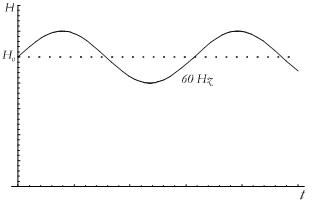
\includegraphics[width=0.3\linewidth]{images/NMR5.jpg}}
    \caption{Applied Magnetic Field varying at 60 Hz}
    \label{fig:AppliedMagneticField}
\end{figure}

When Figures \ref{fig:AbsorptionSignal} and \ref{fig:AppliedMagneticField} are put together, we obtain Figure~\ref{fig:MeasuredSignal}.

\begin{figure}[h]
    \centering
    \href{http://experimentationlab.berkeley.edu/sites/default/files/images/NMR6.gif}{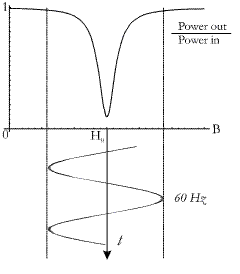
\includegraphics[width=0.3\linewidth]{images/NMR6.png}}
    \caption{Measured signal}
    \label{fig:MeasuredSignal}
\end{figure}

Next is to visualize the resonant ``signal'' shown in Figure~\ref{fig:AbsorptionSignal}. If the input power is kept constant, the resonant signal can be realized as a change in the output power. We will consider the electric field, rather than the power, of the outgoing radiation at the frequency $f_o$ as a function of time and call it the signal. The amplitude of this signal is a measure of the power absorbed in the sample.

\begin{figure}[h]
\begin{minipage}[t]{0.49\textwidth}
    \href{http://experimentationlab.berkeley.edu/sites/default/files/images/NMR7.gif}{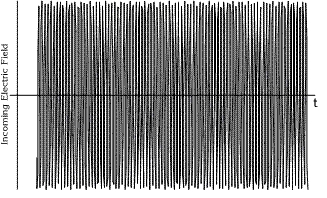
\includegraphics[width=0.9\linewidth,keepaspectratio]{images/NMR7.png}}
    \caption{Amplitude of Incident electric field as a function of time.}
    \label{fig:AmplitudeOfIncidentElectricField}
\end{minipage}\hfill
\begin{minipage}[t]{0.49\textwidth}
    \href{http://experimentationlab.berkeley.edu/sites/default/files/images/330px-NMR8.gif}{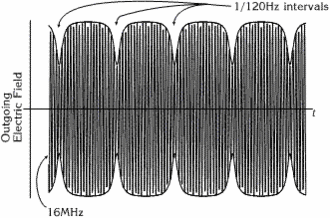
\includegraphics[width=0.9\linewidth,keepaspectratio]{images/330px-NMR8.png}}
    \caption{Amplitude of outgoing electric field as a function of time.}
    \label{fig:AmplitudeOfOutgoingElectricField}
\end{minipage}
\end{figure}

The incident electric field at a frequency of 16 MHz shown in Figure~\ref{fig:AmplitudeOfIncidentElectricField} is now modulated in amplitude at a frequency of 60 Hz as illustrated in Figure~\ref{fig:AmplitudeOfOutgoingElectricField}. The magnitude of the amplitude when plotted in time is a measure of the resonance curve. The function of the detector is to rectify the 16 MHz signal by putting it through a low-pass filter that removes the 16 MHz component but leaves the modulating component at 60 Hz. The resulting signal is sent to an oscilloscope with the sweep frequency set at 60 Hz. If we operate the oscilloscope in the x-y mode, with the x-channel being the modulating magnetic field and the y-channel being the filtered signal, the display of the oscilloscope is the desired resonance curve.

A block diagram with signals at the various stages will be shown in the next section.

To summarize, we place a test tube of a liquid sample in a magnetic field. We then apply electromagnetic radiation at radio frequency to the sample with a nearby transmission coil. We observe the resonance at the Larmor frequency by tuning the input frequency. As the protons precess, they induce an emf in a receiver coil wrapped around the sample. The amplitude of the induced field is at a maximum when the frequency of the applied RF field exactly matches the Larmor frequency. In the detecting circuit we rectify the RF field, filter it to get a DC voltage proportional to the amplitude of the field, and display it on an oscilloscope.

To take data, we set the frequency of the applied RF to the Larmor frequency for the static field produced by the permanent magnet. By superimposing a modulating magnetic field, we then sweep the amplitude of the resulting magnetic field sinusoidally in time at 60 Hz, above and below the static field for resonance (we say that the field is modulated sinusoidally with a frequency of 60 Hz). The final result is a plot of the resonance curve, the amplitude of the detector signal vs. the magnetic field applied to the sample, for a fixed frequency.

\begin{figure}[h]
    \centering
    \href{http://experimentationlab.berkeley.edu/sites/default/files/images/700px-NMR9.gif}{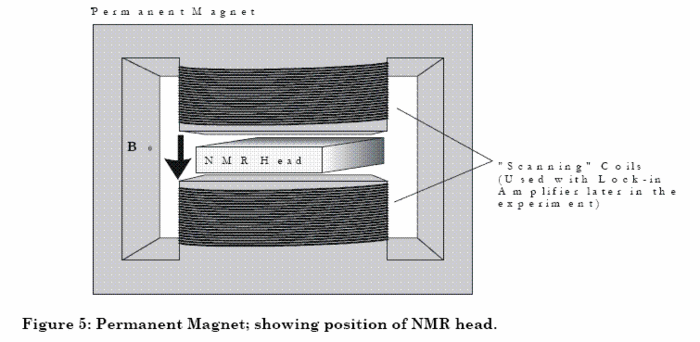
\includegraphics[width=0.5\linewidth]{images/700px-NMR9.png}}
    \caption{}
    \label{fig:700px-NMR9}
\end{figure}

\begin{figure}[h]
    \centering
    \href{http://experimentationlab.berkeley.edu/sites/default/files/images/500px-NMR10.gif}{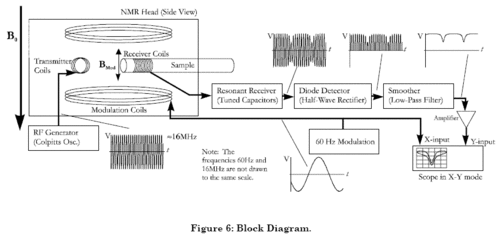
\includegraphics[width=0.5\linewidth]{images/500px-NMR10.png}}
    \caption{Diagrams showing the experimental set up and how the signal is processed.}
    \label{fig:500px-NMR10}
\end{figure}

\begin{figure}[h]
    \centering
    \href{http://experimentationlab.berkeley.edu/sites/default/files/images/500px-NMR11.gif}{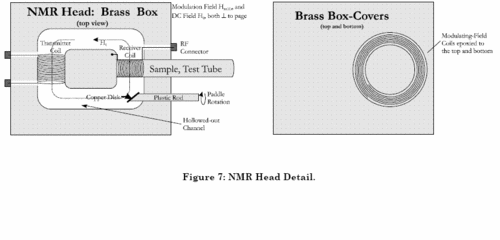
\includegraphics[width=0.5\linewidth]{images/500px-NMR11.png}}
    \caption{Detail of the NMR Head.}
    \label{fig:DetailOfNMRHead}
\end{figure}

\section{Magnet}

In the first part of this experiment we are going to use a $H_0$ about 3.9 kG permanent magnet. The coils of wire wrapped around the poles of the permanent magnet are for the purpose of varying the field at a very low frequency and are needed in the later part of the experiment, where a lock-in amplifier is used.

It is also used with the Lock-in and function generator for sweeping the magnetic field. This is done by using the magnetizing coils wrapped around the magnet iron core.

\section{NMR Head}

Details of the NMR head are shown in Figure~\ref{fig:DetailOfNMRHead}. It is a brass box containing a radio-frequency transmitting coil positioned perpendicularly to a receiving coil into which a test tube contain a sample of protons in H2O or other liquids is inserted. The NMR head is placed between the poles of the permanent magnet. Do \textbf{not} remove this head from the magnet, nor disconnect its cables. Instead, you may examine a spare NMR head on the table.

The top and bottom covers of the NMR head have 7-turn pancake coils which carry varying currents that produce a modulation field $H_\text{mod} \cos(2 \pi f_m t)$, where $f_m$ is 60 Hz. The amplitude $H_\text{mod}$ is controlled from the modulation unit with $H_\text{mod} \approx 1.7$ gauss/amp coming from the modulating current. This is done with a 1.7 amp 60Hz power supply to modulate the field.

\section{NMR Box}

This black box \href{http://experimentationlab.berkeley.edu/sites/default/files/images/NMR31.gif}{\textbf{NMR RF Black Box Circuit Diagram}}

is permanently mounted on the magnet stand and is not to be removed or disassembled; do not remove the cables either. It contains a tunable RF oscillator centered around 16.54x,xxx Mhz, a tunable receiver (left-hand knob), a diode-based detector (right-hand knob), a low-pass filter, and an amplifier for enhancing the detector output. Record this frequency down to 1 Hz resolution for the pulse NMR section.

The oscillator generates an RF signal that produces a magnetic field $H_1\cos(2\pi f t)$ in the sample. The frequency is determined by $1/\sqrt{LC}$ where $L$ and $C$ are the combined inductance and capacitance of the coil in the NMR head, the variable capacitors in the NMR box, and the cables connecting the two. One of the capacitors tunes the circuit to hit resonance at the Larmor frequency. Because the resonant circuit includes inductors in the head and in the cables, as well as capacitors in the NMR box and the cables, touching or moving anything during measurements makes the frequency unstable and introduces lots of noise. Thus, be gentle, and keep your hands off while taking data.

The amplitude of the RF field $H_1$ is controlled by the DC supply voltage $V_1$ to the oscillator. The direction of $H_1$ lies in a plane perpendicular to the DC field $H_0$ of the large permanent magnet. However, the direction relative to the axis of the receiving coil can be adjusted by rotating a copper disk on a ``paddle,'' which controls the phase of the leakage voltage into the receiving coil. Changing the phase enables us to observe either absorption, dispersion or a mixture of the two. In this lab, we will observe adiabatic absorption or dispersion, and non-adiabatic absorption or dispersion modes. See Figures \ref{fig:AdiabaticAbsorption}, \ref{fig:AdiabaticDispersion}, and \ref{fig:NonAdiabaticAbsorption} for examples of these modes.

\begin{figure}[h]
\begin{minipage}[t]{0.31\textwidth}
    \href{http://experimentationlab.berkeley.edu/sites/default/files/images/NMR17.gif}{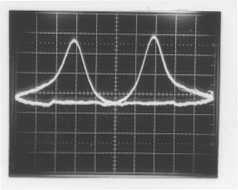
\includegraphics[width=\linewidth]{images/NMR17.png}}
    \caption{Resonance pattern corresponding to Adiabatic (Slow passage) - Absorption ($\sim$ 1.0 Molar Mn$^{++}$in H2O).}
    \label{fig:AdiabaticAbsorption}
\end{minipage}\hfill
\begin{minipage}[t]{0.31\textwidth}
    \href{http://experimentationlab.berkeley.edu/sites/default/files/images/250px-NMR18.gif}{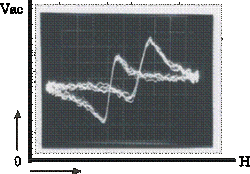
\includegraphics[width=\linewidth]{images/250px-NMR18.png}}
    \caption{Resonance pattern corresponding to Adiabatic (Slow Passage) - Dispersion ($\sim$ 1.0 Molar Mn$^{++}$in H2O).}
    \label{fig:AdiabaticDispersion}
\end{minipage}\hfill
\begin{minipage}[t]{0.31\textwidth}
    \href{http://experimentationlab.berkeley.edu/sites/default/files/images/NMR19.gif}{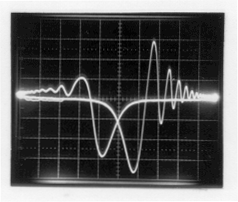
\includegraphics[width=\linewidth]{images/NMR19.png}}
    \caption{Resonance pattern corresponding to Non-Adiabatic passage - Absorption ($\sim$ 0.1 Molar Mn$^{++}$in H2O).}
    \label{fig:NonAdiabaticAbsorption}
\end{minipage}
\end{figure}

\emph{\textbf{Check Point: show the above pictures you have setup to  the professor or GSI.}}

\section{Block Diagram}

Refer to Figure A for the NMR Block Diagram:

The NMR head is placed in the DC field $H_0 \approx$ 3800 gauss of a large permanent magnet. The simplest method for observing NMR is to sweep the magnetic field through resonance at 60 Hz by superimposing a modulating $H_\text{mod}$ on $H_0$. Also, it is helpful to display the NMR signal $V_\text{ac}$as the y-input of an oscilloscope and the 60-Hz phase shifted sine wave from the modulation unit as the x-input.

The signal from the NMR box is amplified by the SRS 560 amplifier which is used to limit the upper and lower pass frequency (typically 10 kHz and 3 Hz), thereby rejecting unwanted frequencies and improving the visibility of the desired signal. The Fluke frequency counter is used to read the NMR oscillator frequency without perturbing the oscillator.

The coils wrapped around the pole pieces of the magnet were initially used to magnetize the Alnico alloy of the poles, but are no longer needed or used for this purpose. Instead, they are used in the second part of the experiment for superimposing on $H_0$ a small monotonically increasing field $H_2(t)$ generated by the Function Generator (the field will vary as a triangle function). The field reaches a maximum amplitude of about 60 gauss. The triangle frequency can be as small as 0.01 Hz, thereby enabling slow, repetitive scanning in one direction through the magnetic resonance. The Lock-in amplifier (see section on Lock-ins) is used for recording the derivative of the NMR signal.

\section{Samples}

\emph{\textbf{Check Point: Show the professor or GSI your CW setup with picture on scope. What is the line width for Glycerin? For water?}}

To observe resonance of the proton, use the prepared set of samples of H$_2$O + MnCl$_2$4H$_2$O with yellow mylar tape on the top. The Mn molarity (M) ranges from M = 3.3, 1.0, 0.33, ..., to $10^{-5}$ moles of MnCl$_2$4H$_2$O per liter of solution, and gives a wide range of relaxation times. A one molar sample contains 19.7 grams of MnCl$_2$4H$_2$O in 100 cc of mixed solution. Other useful samples are glycerin with a small amount of FeCl$_3$, and pure H$_2$O. For F$^{19}$ we are going to use Teflon rods. Samples should be tightly stopped and contain no air bubbles. Be careful not to drop or open the test tubes. Call for the staff if any solution comes out of the test tubes.

\section{NMR Lock In Amplifier}

A lock-in amplifier has various capabilities, one of which is the detection of ac signals of incredibly low signal-to-noise ratios. This capability results from the filtering mechanism it employs, which creates incredibly narrow passbands (think 0.01 Hz). How is this possible, you ask? The filtering technique involves two essential components: a mixer and low-pass filter.

A mixer takes in two waves, $f_1(x) = V_a\sin(ax)$ and $f_2(x) = V_b\sin(bx)$, of frequency $a$ and $b$ respectively. Its output is the \emph{product} of those two waves. Recall the trig identity for the product of two waves:
\begin{align*}
f_1(x) f_2(x) &= V_a V_b \sin(ax)\sin(bx) \\
&= \frac{1}{2} V_a V_b(\cos((a-b)x) - \cos((a+b)x))
\end{align*}
Now consider the special case where both input waves have the same frequency, i.e. $a = b$. Then our mixer output is given by:
\[
\frac{1}{2} V_a V_b(\cos((a-a)x) - \cos((a+a)x))
    = \frac{1}{2}V_a V_b - \frac{1}{2} V_a V_b \cos(2ax)
\]
Note that the in this case, the output is simply the sum a DC signal with amplitude $\frac{1}{2} V_a V_b$ and an AC signal with frequency $2a$. If we low-pass filter the mixer output, we get rid of the AC signal, leaving us with just the DC signal. If we know $V_b$, then we can calculate $V_a$ by measuring the DC amplitude and dividing by $V_b/2$.

This analysis neglects, however, the possibility of a phase shift between the two waves. In fact, if we include the possibility of a phase shift, then the DC output (after low-pass filtering), also depends on the phase shift. It turns out that the amplitude of the DC signal acquires a factor of $\cos(\Delta \phi)$, where $\Delta \phi$ represents the phase difference of the two waves. For this reason, a feedback circuit is added to maintain a constant phase difference of 0 degrees between the two waves.

\subsection{Part of Lock-In Manual model SRS 830}

Lock-in amplifiers are used to detect and measure very small AC signals - all the way down to a few nanovolts! Accurate measurements may be made even when the small signal is obscured by noise sources many thousands of times larger.

Lock-in amplifiers use a technique known as phase-sensitive detection to single out the component of the signal at a specific reference frequency AND phase. Noise signals at frequencies other than the reference frequency are rejected and do not affect the measurement.

\textbf{Note on lock-in amplifier: To reset the lock-in, hold the setup key when the power is on.}

Full Manual \href{http://physics111.lib.berkeley.edu/Physics111/Equipment\_Manuals/SRS/SR830m.pdf}{\textbf{Lock-in}}

\subsection{Why use a lock-in?}

Lock-in information \href{http://physics111.lib.berkeley.edu/Physics111/Reprints/NMR/Lock-in-Amp.pdf}{\textbf{Lock-in Amp}} About a Lock-in \href{http://physics111.lib.berkeley.edu/Physics111/Reprints/NMR/About-Lock-Ins.pdf}{\textbf{Lock-ins}}

Let's consider an example. Suppose the signal is a 10 nV sine wave at 10 kHz. Clearly some amplification is required. A good low-noise amplifier will have about 5 nV/$\sqrt{\text{Hz}}$ of input noise. If the amplifier bandwidth is 100 kHz and the gain is 1000, then we can expect our output to be 10 $\mu$V of signal (10 nV $\times$ 1000) and 1.6 mV of broadband noise (5nV/$\sqrt{\text{Hz}}$ $\times$ $\sqrt{100}$ kHz $\times$ 1000). We won't have much luck measuring the output signal unless we single out the frequency of interest.

If we follow the amplifier with a band pass filter with a $Q$ = 100 (a VERY good filter) centered at 10 kHz, any signal in a 100 Hz bandwidth will be detected (10 kHz/$Q$). The noise in the band pass filter will be 50 $\mu$V (5 nV/$\sqrt{\text{Hz}} \times \sqrt{100}$ Hz $\times$ 1000) and the signal will still be 10 $\mu$V. The output noise is much greater than the signal and an accurate measurement can not be made. Further gain will not help the signal to noise problem.

Now try following the amplifier with a phase sensitive detector (PSD). The PSD can detect the signal at 10 kHz with a bandwidth as narrow as 0.01 Hz! In this case, the noise in the detection bandwidth will be only 0.5 $\mu$V (5 nV/$\sqrt{\text{Hz}} \times \sqrt{.01}$ Hz $\times$ 1000) while the signal is still 10 (V. The signal to noise ratio is now 20 and an accurate measurement of the signal is possible.

\subsection{What is phase-sensitive detection?}

Lock-in measurements require a frequency reference. Typically an experiment is excited at a fixed frequency (from an oscillator or function generator) and the lock-in detects the response from the experiment at the reference frequency. In the diagram below, the reference signal is a square wave at frequency $\omega_r$. This might be the sync output from a function generator. If the sine output from the function generator is used to excite the experiment, the response might be the signal waveform shown below. The signal is
\[
    V_\text{sig}\sin(\omega_rt + \theta_\text{sig}) \text{ where } V_\text{sig} \text{ is the signal amplitude.}
\]

\begin{figure}[h]
    \centering
    \href{http://experimentationlab.berkeley.edu/sites/default/files/images/300px-NMR33.jpg}{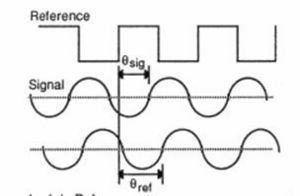
\includegraphics[width=0.5\linewidth]{images/300px-NMR33.jpg}}
    \caption{Lock-In Reference}
    \label{fig:300px-NMR33}
\end{figure}

The SR830 generates its own sine wave, shown as the lock-in reference to the right. The lock-in reference is $V_L \sin(\omega_Lt + \theta_\text{ref})$.

The SR830 amplifies the signal and then multiplies it by the lock-in reference using a phase-sensitive detector or multiplier. The output of the PSD is simply the product of two sine waves.
\begin{align*}
    V_\text{psd} &= V_\text{sig} V_L \sin (\omega_rt + \theta_\text{sig}) \sin (\omega_Lt + \theta_\text{ref}) \\
    &= \frac{1}{2} V_\text{sig} V_L \cos ([\omega_r - \omega_L ]t + \theta_\text{sig} - \theta_\text{ref}) - \frac{1}{2} V_\text{sig} V_L \cos ([\omega_r + \omega_L ]t + \theta_\text{sig} + \theta_\text{ref})
\end{align*}
The PSD output is two AC signals, one at the difference frequency $(\omega_r - \omega_L)$ and the other at the sum frequency $(\omega_r + \omega_L)$.

If the PSD output is passed through a low pass filter, the AC signals are removed. What will be left? In the general case, nothing. However, if $\omega_r = \omega_L$, the difference frequency component will be a DC signal. In this case, the filtered PSD output will be
\[
    V_\text{psd} = \frac{1}{2} V_\text{sig} V_L \cos(\theta_\text{sig} - \theta_\text{ref})
\]
This is a very nice signal - it is a DC signal proportional to the signal amplitude.

\subsection{Narrow band detection}

Now suppose the input is made up of signal plus noise. The PSD and low pass filter only detect signals whose frequencies are very close to the lock-in reference frequency. Noise signals at frequencies far from the reference are attenuated at the PSD output by the low pass filter (neither $\omega_\text{noise} - \omega_\text{ref}$ nor $\omega_\text{noise} + \omega_\text{ref}$ are close to DC). Noise at frequencies very close to the reference frequency will result in very low frequency AC outputs from the PSD ($|\omega_\text{noise} - \omega_\text{ref}|$ is small). Their attenuation depends upon the low pass filter bandwidth and roll-off. A narrower bandwidth will remove noise sources very close to the reference frequency, a wider bandwidth allows these signals to pass. The low pass filter bandwidth determines the bandwidth of detection. Only the signal at the reference frequency will result in a true DC output and be unaffected by the low pass filter. This is the signal we want to measure.

\subsection{Where does the lock-in reference come from?}

We need to make the lock-in reference the same as the signal frequency, i.e. $\omega_r = \omega_L$. Not only do the frequencies have to be the same, the phase between the signals can not change with time, otherwise $\cos(\theta_\text{sig} - \theta_\text{ref})$ will change and Vpsd will not be a DC signal. In other words, the lock-in reference needs to be phase-locked to the signal reference.

Lock-in amplifiers use a phase-locked-loop (PLL) to generate the reference signal. An external reference signal (in this case, the reference square wave) is provided to the lock-in. The PLL in the lock-in locks the internal reference oscillator to this external reference, resulting in a reference sine wave at $\omega_r $ with a fixed phase shift of $\theta_\text{ref}$ Since the PLL actively tracks the external reference, changes in the external reference frequency do not affect the measurement.

\subsection{All Lock-In Measurements Require a Reference Signal}

In this case, the reference is provided by the excitation source (the function generator). This is called an external reference source. In many situations, the SR830's internal oscillator may be used instead. The internal oscillator is just like a function generator (with variable sine output and a TTL sync) which is always phase-locked to the reference oscillator.

\subsection{Magnitude and Phase}

Remember that the PSD output is proportional to $V_\text{sig} \cos \theta$ where $\theta = (\theta_\text{sig} - \theta_\text{ref})$. $\theta$ is the phase difference between the signal and the lock-in reference oscillator. By adjusting $\theta_\text{ref}$ we can make $\theta$ equal to zero, in which case we can measure Vsig$(\cos \theta = 1)$. Conversely, if $\theta$ is 90$^\circ$, there will be no output at all. A lock-in with a single PSD is called a single-phase lock-in and its output is $V_\text{sig} \cos \theta$.

This phase dependency can be eliminated by adding a second PSD. If the second PSD multiplies the signal with the reference oscillator shifted by 90$^\circ$, i.e. $V_L \sin(\omega_Lt + \theta_\text{ref} + 90)$, its low pass filtered output will be
\[
    V_\text{psd2} = \frac{1}{2} V_\text{sig} V_L \sin(\theta_\text{sig} - \theta_\text{ref}) \sim V_\text{sig} \sin \theta
\]
Now we have two outputs, one proportional to cos$\theta$ and the other proportional to sin$\theta$. If we call the first output $X$ and the second $Y$,
\[
    X = V_\text{sig} \cos \theta Y = V_\text{sig} \sin \theta
\]

these two quantities represent the signal as a vector relative to the lock-in reference oscillator. $X$ is called the 'in-phase' component and Y the 'quadrature' component. This is because when $\theta$ = 0, $X$ measures the signal while $Y$ is zero.

By computing the magnitude (R) of the signal vector, the phase dependency is removed.
\[
    R = (X^2 + Y^2)^{1/2} = V_\text{sig}
\]
R measures the signal amplitude and does not depend upon the phase between the signal and Lock-in reference.

A dual-phase lock-in, such as the SR830, has two PSD's, with reference oscillators 90$^\circ$ apart, and can measure $X$, $Y$ and $R$ directly. In addition, the phase (between the signal and lock-in reference, can be measured according to
\[
    \theta = \tan^{-1} \left(\frac{Y}{X} \right)
\]

\subsection{What Does a Lock-In Measure?}

So what exactly does the SR830 measure? Fourier's theorem basically states that any input signal can be represented as the sum of many, many sine waves of differing amplitudes, frequencies and phases. This is generally considered as representing the signal in the ``frequency domain''. Normal oscilloscopes display the signal in the ``time domain''. Except in the case of clean sine waves, the time domain representation does not convey very much information about the various frequencies which make up the signal.

\subsection{What Does the SR830 Measure?}

The SR830 multiplies the signal by a pure sine wave at the reference frequency. All components of the input signal are multiplied by the reference simultaneously. Mathematically speaking, sine waves of differing frequencies are orthogonal, i.e. the average of the product of two sine waves is zero unless the frequencies are EXACTLY the same. In the SR830, the product of this multiplication yields a DC output signal proportional to the component of the signal whose frequency is exactly locked to the reference frequency. The low pass filter which follows the multiplier provides the averaging which removes the products of the reference with components at all other frequencies.

The SR830, because it multiplies the signal with a pure sine wave, measures the single Fourier (sine) component of the signal at the reference frequency. Let's take a look at an example. Suppose the input signal is a simple square wave at frequency 'f'. The square wave is actually composed of many sine waves at multiples of 'f' with carefully related amplitudes and phases. A 2V pk-pk square wave can be expressed as
\[
    S(t) = 1.273 \sin(\omega t) + 0.4244 \sin(3 \omega t) + 0.2546 \sin(5 \omega t) + ...
\]
where $\omega = 2 \pi f$. The SR830, locked to `f' will single out the first component. The measured signal will be $1.273 \sin(\omega t)$, not the 2V pk-pk that you'd measure on a scope.

In the general case, the input consists of signal plus noise. Noise is represented as varying signals at all frequencies. The ideal lock-in only responds to noise at the reference frequency. Noise at other frequencies is removed by the low pass filter following the multiplier. This "bandwidth narrowing. is the primary advantage that a lock-in amplifier provides. Only inputs at frequencies at the reference frequency result in an output.

\subsection{RMS or Peak?}

Lock-in amplifiers as a general rule display the input signal in Volts RMS. When the SR830 displays a magnitude of 1V (rms), the component of the input signal at the reference frequency is a sine wave with an amplitude of 1 Vrms or 2.8 V pk-pk.

Thus, in the previous example with a 2 V pk-pk square wave input, the SR830 would detect the first sine component, $1.273 \sin(\omega t)$. The measured and displayed magnitude would be 0.90 V (rms)$\left(\frac{1}{\sqrt{2}} \times 1.273 \right)$.

\subsection{Degrees or Radians?}

In this discussion, frequencies have been referred to as $f$ (Hz) and $\omega$ ($2 \pi f$ radians/sec). This is because people measure frequencies in cycles per second and math works best in radians. For purposes of measurement, frequencies as measured in a lock-in amplifier are in Hz. The equations used to explain the actual calculations are sometimes written using (to simplify the expressions.

Phase is always reported in degrees. Once again, this is more by custom than by choice. Equations written as $\sin(\omega t + \theta)$ are written as if $\theta$ is in radians mostly for simplicity. Lock-in amplifiers always manipulate and measure phase in degrees.

\subsection{The Functional SR830}

\begin{figure}[h]
    \centering
    \href{http://experimentationlab.berkeley.edu/sites/default/files/images/500px-NMR34.jpg}{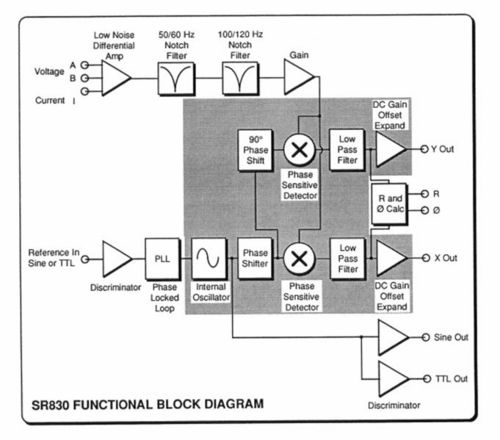
\includegraphics[width=0.5\linewidth]{images/500px-NMR34.jpg}}
    \caption{}
    \label{fig:500px-NMR34}
\end{figure}

The functional block diagram of the SR830 DSP Lock-In Amplifier is shown below. The functions in the gray area are handled by the digital signal processor (DSP). The DSP aspects of the SR830 are covered in the SR830 manual. They are described as they come up in each functional block description. (See Section three (3) in the SR 830 Manual)

\section{Digital Oscilloscope:}

This experiment uses a Digital Storage oscilloscope in order to examine the weak resonance signals. See the included manual located in the reprints on how to use the digital storage scope. The output signal is also connected to the computer so that the data could be transferred to the computer and stored for later use. The instructions on how to transfer the data to the computer are located in a section at the end of this write-up.

\begin{figure}[h]
    \centering
    \href{http://experimentationlab.berkeley.edu/sites/default/files/images/500px-NMRblockdiagram.jpg}{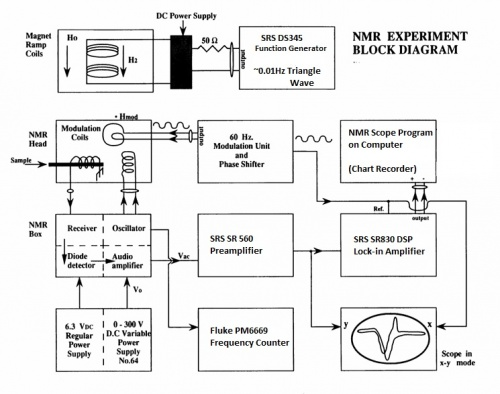
\includegraphics[width=0.6\linewidth]{images/500px-NMRblockdiagram.jpg}}
    \caption{NMR Block Diagram}
    \label{fig:500px-NMRblockdiagram}
\end{figure}

\section{Procedures}

\subsection{Getting Started}

\begin{enumerate}
    \item HEATHKIT POWER SUPPLY. Flip the POWER switch to STANDBY and wait 1 minute; then switch to ON. Set the METER SWITCH to the RIGHT. Set the amplitude of the RF field by adjusting the B+ OUTPUT knob to 150 volts, as read by the voltmeter.

    \item On the $H_\text{mod}$ magnetic field modulation control panel. Flip POWER and SWEEP ON switches up. Turn the AMPLITUDE ADJUST knob to its maximum CW position to maximize the modulation of the field. This sends about 1.7 amp at 60 HZ to the modulation coils; this current generates a magnetic field of about 2.9 gauss.

    \item The PHASE ADJUST knob on the $H_\text{mod}$ panel changes the phase of the modulation signal sent to the x-input of the scope relative to the signal sent to the modulation coils, and hence relative to the detected output signal sent to the y-input of the scope. In short, it changes the phase between the x and y signals. No need to set it at this time.

    \item PRE-AMP, Stanford Research Systems Model SR 560. Turn the unit on and plug the AUDIO OUTPUT from the back of the NMR box into INPUT A and make sure that the DC /GND/AC switch next to the A input is in the AC position. Note that if you suddenly lose your original signal while you are making various adjustments - if your scope trace goes flat - you should push the OV LD overload recovery switch down. Set the gain to 50, the LF ROLL-OFF to 3 Hz, and the HF ROLL-OFF to 10K. You will probably have to adjust these later to make your signal as clean as possible without losing any of its major features.

    \item Turn on the RF POWER SUPPLY.

    \item Turn on the frequency counter (Fluke PM6669) and the oscilloscope. Connect the FREQUENCY MONITOR on the back of the NMR box to the input of the frequency counter. Put the scope in the x-y mode. Then connect the PHASE ADJUST to the x-input of the scope and the PRE-AMP output to the y-input of the scope.

    \item Now you're ready to go. Insert a glycerin sample into the NMR HEAD and find the resonance signal by doing the following. Look up in the \href{http://dev-physicsadv.pantheon.berkeley.edu/sites/default/files/images/NMR32.jpg}{\textbf{NMR Frequency TABLE}} of the manual - the NMR frequency for H$^1$ in a 10 kilogauss field. Knowing this number and that our $H_0$ is about 3.8 kG, calculate the approximate NMR frequency for our set-up (around 16.1xxxxx Mhz). Turn the TRANS FREQ knob on the NMR BOX until the counter reads this value. Now adjust the receiver coil to observe the resonance by adjusting the CR control so that the receiver frequency matches that of the transmitter. Start with it at the fiducial mark.

    \begin{figure}[h]
    \begin{minipage}[t]{0.33\textwidth}
        \href{http://experimentationlab.berkeley.edu/sites/default/files/images/NMR21.gif}{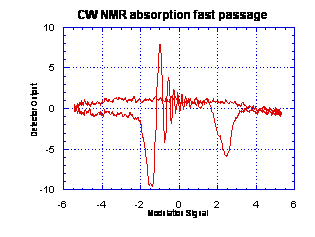
\includegraphics[width=0.95\linewidth,keepaspectratio]{images/NMR21.png}}
        \caption{0.1 Molar Mn$^{++}$ in H2O}
        \label{fig:TenthMolarMn}
    \end{minipage}\hfill
    \begin{minipage}[t]{0.31\textwidth}
        \href{http://experimentationlab.berkeley.edu/sites/default/files/images/NMR22.gif}{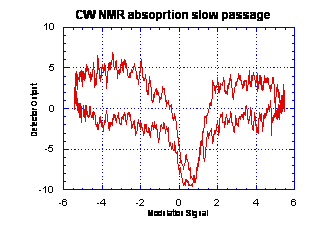
\includegraphics[width=\linewidth,keepaspectratio]{images/NMR22.png}}
        \caption{1 Molar Mn$^{++}$ in H2O}
    \end{minipage}\hfill
    \begin{minipage}[t]{0.31\textwidth}
        \href{http://experimentationlab.berkeley.edu/sites/default/files/images/NMR23.gif}{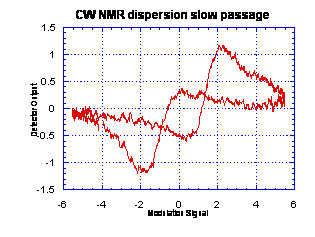
\includegraphics[width=\linewidth,keepaspectratio]{images/NMR23.png}}
        \caption{1 Molar Mn$^{++}$ in H2O}
    \end{minipage}
    \end{figure}

    Make sure that the amplitude is ``peaked'' on the NMR box. Adjust the peak knob until the maximum microampere reading is shown. This will have to be done for every sample used. Slowly vary the frequency around the value you calculated above. You should be able to find the resonance, and your signal should look like Figure~\ref{fig:TenthMolarMn}. Note that the resonance condition is very sensitive to frequency; so go slowly. Once you have found it, ``peak-up'' your signal by readjusting CR on the NMR BOX for maximizing the signal. If you don't find a signal after you've fussed with everything, ask for help. Once resonance is found, adjust the x-axis of the scope until both edges of the signal are visible on the screen. Vary the frequency so that the resonance signal goes barely off the edge to the left of the screen, and record the frequency. Do the same for the right side of the screen. Subtract the frequencies, and the difference will be the scanning frequency range. You will not need to scan past this range when searching for resonance for any sample, once the signal is found (It should be $\sim$90kHz).
    
    Move the NMR HEAD around gently in the gap until you have maximized the number of ``wiggles'' and minimized the line width. This will place the head in the most uniform or homogeneous region of the magnet, and you want to keep it there. Once you have set the position for the day, don't change it. Some of your calculations depend on the field being the same for successive measurements. Repeat this procedure each day when you first come to the lab, since other people may have moved the NMR head from where you have determined to be the best.

    \item Read over the REPORT section to be sure you take all the necessary data. Read the information described in section at the end of this write-up on how to transfer data to the computer.
\end{enumerate}

\subsection{Taking Data}

\begin{enumerate}
    \item By using the glycerin sample you can find a narrow line (that is, a sharp resonance) in the homogeneous region of the magnet. Once the resonance is observed, tune the phase adjust knob until the two peaks are symmetric about the midpoint of the $H_\text{mod}$ trace on the scope, for both slow passage and non-adiabatic passage conditions. Measure the resonant frequency and hence (by knowing γ) the magnetic field to high precision. It is a standard technique to use NMR to determine the magnetic field strength precisely.

    \item By recalling that $\Delta f / f = \Delta H / H$, where $f$ is the frequency and $H$ is the magnetic field, you can devise a method of calibrating (in gauss/div) the field axis of the oscilloscope. Then you can transfer the data of the four modes (absorption/dispersion; slow passage/non-adiabatic passage) to the computer.
    
    \item Replace the glycerin sample with a 0.01M Mn$^{++}$sample; again this signal should look like Figure 8. Download the data of this non-adiabatic rapid-passage absorption mode to the computer. (See REPORT, \#3.) Now insert a more highly doped sample, 1M Mn$^{++}$. The paramagnetic Mn$^{++}$ions relax the proton spins and the signal is closely resembled the one of a slow passage absorption mode. By further rotating the paddles you should be able to get a signal like Fig. 10, approximately a slow passage dispersion mode. You may have to increase $V_1$ to see this.
    
    \item For observing the F$^{19}$ resonance we use a Teflon rod. Note that the F$^{19}$ resonance is a little harder to find. Using the same procedures as for H$^1$, find the resonance curves for F$^{19}$. Accurately measure the NMR frequency ratio of F$^{19}$ to H$^1$. To do that, measure $f(\text{H}^1)$ and $f(\text{F}^{19})$ each a number of times under identical conditions.
    
    \item Lock-in Amplifier Operation: For fine tuning the NMR resonance, we can leave the frequency $f$ and all the other parameters fixed and optimized, and vary the ``total-DC'' magnetic field by adding a small field $H_2$ with the output of the \href{https://youtu.be/PrM8DHFOFS0}{\textbf{SRS DS345 generator}} driving the wire coils. The following diagrams show what this change does to the signal. See Figure~\ref{fig:LockInAmplifierSignals}.
\end{enumerate}

\begin{figure}[h]
    \centering
    \href{http://experimentationlab.berkeley.edu/sites/default/files/images/NMR25.gif}{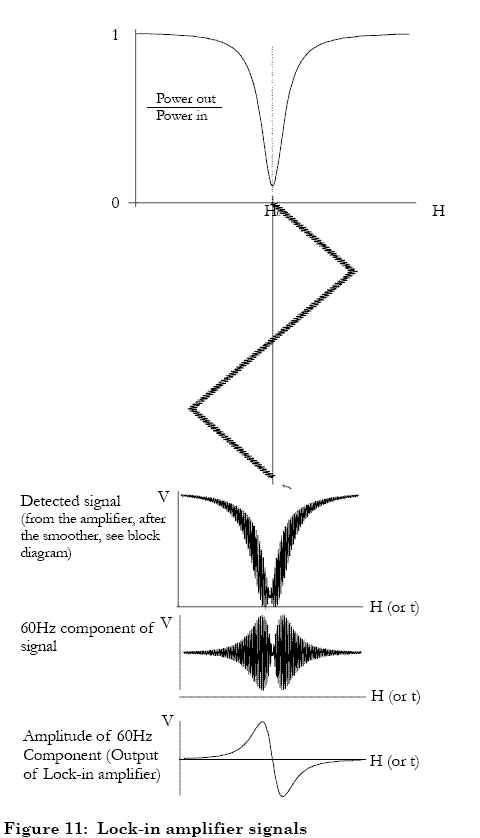
\includegraphics[width=0.5\linewidth]{images/NMR25.png}}
    \caption{Lock-in amplifier signals}
    \label{fig:LockInAmplifierSignals}
\end{figure}

Read ``Basic Introduction to Lock-in Amplifiers'' in the \href{http://www.advancedlab.org/mediawiki/index.php/NMR\_Lock\_In\_Amplifier}{\textbf{Lock-in Amplifier}}, and the manual of the Stanford Research Systems Model SR 830DSP Lock-in Amplifier (copied in reprints). In this apparatus, the lock-in amplifier records the derivative $dV_\text{ac}(H)/dH$ of the NMR signal as the frequency sweeps slowly through the resonance by varying the field $H_2$ with the signal generator. The signal-to-noise ratio can be 100$\times$ larger than that observed with the oscilloscope. This method is used to find and record weak signals. It also provides a convenient way to record the line width $\delta H$ of a signal.

As usual, getting started is not trivial. First you need to have a good signal on the oscilloscope. Then turn on the power supply of the magnet (Hewlett Packard E3615A DC Power Supply), the lock-in amplifier, and the function generator. Set the function generator to give a triangle wave with an initial frequency of .05 Hz and 1 $V_\text{pp}$ amplitude. Check out the OFFSET control to adjust the voltage where the triangle wave will be centered. The output of the signal generator goes to the input of the HP E3615A, located in the back of the unit.

You want to sweep the field as shown in Figure~\ref{fig:LockInAmplifierSignals}. Unfortunately, the power supply of the magnet does not generate a negative current and the sweep starts at the resonance field Ho. Consequently, the sweep is not symmetrical, and half the resonance curve is lost. In order to compensate for this, we must adjust the offset of the power supply so that it will generate a symmetric sweep using only positive currents. Additionally, the RF frequency must change to a higher value in order to put the resonance at the middle of the triangular sweep. This means the resonance curve will no longer be at the center of the of the scan like in the previous part of the experiment but will be pushed off to one end instead. How much does the RF need to be adjusted? Experiment to find out.

Set the lock-in controls as follows:

\begin{enumerate}
    \item Phase - 0;

    \item zero offset, switch off;

    \item Time Constant - 1 sec.
\end{enumerate}

T-split the phase adjust on the $H_\text{mod}$ panel and connect one of the BNC cables to the phase input (ref) on the Lock-in and the other to the X-input on the DAQ box. It would be useful to put a T on each channel of the oscilloscope, so that you can run the inputs to the scope and then just simply connect the channels on the scope to the DAQ, so that you can easily monitor the traces just by viewing the scope.

Now how do you start? Turn the amplitude of $H_\text{mod}$ way down, to about 10$\sim$20\% of its original value. Refer to the diagrams above. For the first part of the experiment, $H_\text{mod}$ was large; for this part it must be small (but not too small, how come?). Once things are working, adjust the amplitude to peak the signal. With the pre-amplifier hooked up to the Y channel of the scope, you should see the resonance curve sweeping across the face of the scope, and off the end. A few seconds later it should return and sweep across and off the other end. You want the sweep to be symmetrical and off the screen on both sides. I.e., adjust the offset and amplitude on the signal generator to make the resonance peaks go off the right and left hand sides of the oscilloscope, and that the amount of time spent off the screen is minimal and even for both sides. The voltage on the magnet power supply should be going from zero up and back again. If you are monitoring the signal generator output on another oscilloscope, the horizontal line should go up and down from zero. When it is halfway, the resonance curve should be in the center of the scope.

Once a good sweep is established, disconnect the pre-amplifier from the Y-input and connect the Ch. 1 output of the lock-in to the Y-input of the DAQ box and flip the switch to CW mode. Take a strip chart recording with a scan rate of 20.00.

For the H2O samples with molarity of 3, 1, 0.3, 0.1, 0.03 molar Mn$^{++}$, adjust the mode to absorption and set $H_\text{mod}$ small, $\sim$1/8 the line width; this takes the derivative (see Ref.~\cite{Liboff}, p. 51). Adjust the lock-in amplifier and record the derivative with the computer.

Figure~\ref{fig:OutputFor33Molar} shows a typical result for a 0.33 Molar  Mn$^{++}$ sample. (Settings used were H-MOD amplitude adjust 15, Signal generator frequency 0.012Hz, amplitude 0.40, offset 2.07. Lock-in settings: 1s time constant, 6 dB, DC coupling, ground, and Ch.1 Output on ``display''). By scanning more slowly, one can get a good measure of the line width H between the peaks. To measure the signal-to-noise ratio (S/N), one can increase the input gain by, say, 10x or more to record the RMS noise off resonance.

Figure~\ref{fig:OutputForGlycerin} shows a screenshot of the chart recording for glycerin. The settings were identical to the ones listed above for Mn$^{++}$.

\begin{figure}[h]
\begin{minipage}{0.49\textwidth}
    \href{http://experimentationlab.berkeley.edu/sites/default/files/images/500px-0_33MMnchart.jpg}{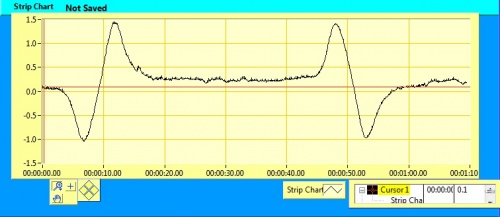
\includegraphics[width=\linewidth,keepaspectratio]{images/500px-0_33MMnchart.jpg}}
    \caption{Protons in 0.33M Mn$^{++}$ in H2O. Output from the chart recorder in Labview.}
    \label{fig:OutputFor33Molar}
\end{minipage}\hfill
\begin{minipage}{0.49\textwidth}
    \href{http://experimentationlab.berkeley.edu/sites/default/files/images/500px-Glycerinchart.jpg}{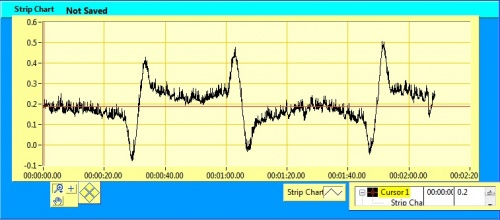
\includegraphics[width=\linewidth,keepaspectratio]{images/500px-Glycerinchart.jpg}}
    \caption{Output from the chart recorder in Labview for glycerin.}
    \label{fig:OutputForGlycerin}
\end{minipage}
\end{figure}

\emph{\textbf{Check Point: Show the above trace to the professor or GSI for sign off.}}

Traces recorded for Mn$^{++}$ samples tend to look nicer (like the ones above). A good trace will peak and return to almost the same level as before the peak, like the traces above. For compounds such as glycerin, there will be a gap between where it starts the peak and where it returns to. Try to minimize this gap by adjusting the H-MOD amplitude adjust, and the frequency of the signal generator.

\section{NMR Scope Program}

\emph{\textbf{How to transfer data from the scope to the computer.}}

\emph{\textbf{Setup:}}

First we need to make a connection between the computer and the oscilloscope. To do that, locate the aluminum box labeled \textbf{Computer Interface Unit}. Connect the \emph{X input (X/Trig CW)} with the knob on the $H_\text{mod}$ corresponding to the sign ``\emph{PHASE OUT}''. Now, depending on which part of the CW NMR you are doing, either connect the \emph{Y input (Y In)} with the output of \textbf{PRE-AMP} or connect the \emph{Y input} with the output of the \emph{Lock-in}. The other port of the interface unit should have a 50-ohm termination. Don't forget to turn on the \emph{Computer Interface Unit} and flip the mode switch to \emph{CW}.

Now we are ready to use the computer to transfer the data.

\emph{\textbf{NMR Scope Program}}

The program we are going to use to transfer the data is called \textbf{NMR Scope2.0.vi}. To get familiar with the program you might want to follow the following simple exercise.

On the desktop you will find an icon \textbf{NMR Scope2.0.vi}. Double click on that icon to open up the program. You will see the following window:

\begin{figure}[h]
    \centering
    \href{http://experimentationlab.berkeley.edu/sites/default/files/images/NMR35.jpg}{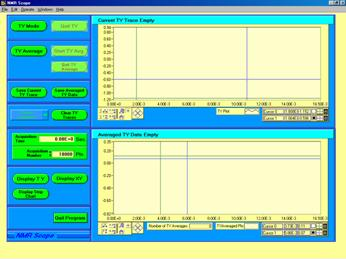
\includegraphics[width=0.5\linewidth]{images/NMR35.jpg}}
    \caption{}
    \label{fig:NMR35}
\end{figure}

\begin{enumerate}
    \item First select the type of experiment you are doing. There are two options: \emph{Pulsed NMR Rising Edge Triggering} and \emph{CW NMR Falling Edge Triggering}

    \item At the bottom left corner you will see three buttons: \textbf{Display TY}(time plotted on the x-axis), \textbf{Display XY}, and \textbf{Display Strip Chart}. The latter one will be used later in the experiment. For now, press either \textbf{Display TY} or \textbf{Display XY} button.
    
    \item To see the signal press the \textbf{TY Mode} or the \textbf{XY Mode}, depending on the previous choice you have made. You should now see a signal in the upper right chart. This is what it might look like:
    
    \begin{minipage}{0.49\linewidth}
        \centering
        \href{http://experimentationlab.berkeley.edu/sites/default/files/images/NMR36.jpg}{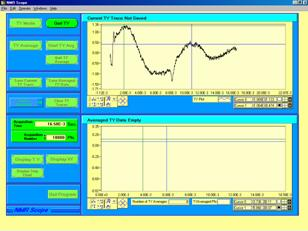
\includegraphics[width=\linewidth]{images/NMR36.jpg}} \\
        TY Mode
    \end{minipage}\hfill
    \begin{minipage}{0.49\linewidth}
        \centering
        \href{http://experimentationlab.berkeley.edu/sites/default/files/images/NMR37.jpg}{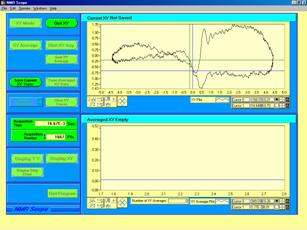
\includegraphics[width=\linewidth]{images/NMR37.jpg}} \\
        XY Mode
    \end{minipage}
    
    \item To zoom in on the signal, press the magnifying glass located directly below the graph. Here, you will find several zoom options to zoom in on the entire graph, portions of the graph, etc. To manually drag the graph to display different portions of the trace, click the hand icon located next to the magnifying glass.
    
    \item To stop the signal, press \textbf{Quit TY}, or \textbf{Quit XY} signal accordingly.
    
    \item To save the data, press \textbf{Save Current TY/XY Traces}. Save the data as a .dat file format.
    
    \item To clear the graph, press \textbf{Clear TY/XY Traces}.
\end{enumerate}

\textbf{Note: you can actually copy the graph and print it separately. Right click anywhere on the graph and press Copy Data. This temporary stores the image on the computer and you can paste it in most programs such as word or excel.}

\emph{\textbf{Averaging the Data:}}

We can also ``average out'' the signal to get a smother line. The program takes multiple samples over time and takes the average. You can average the data in wither mode: TY or XY. After choosing the mode, you might want to go over the following steps:

\begin{enumerate}
    \item Press \textbf{TY/XY Average}. The window comes up asking if you want to ``AutoSave the data.'' If you wish to do so, press yes and it will prompt you to save it. Otherwise, press no. In either case, you will get a window, asking to ``Chose Acquisition Points.'' Just press ok. In the middle to the left of the program window you can set either the acquisition time or acquisition points. By default they are set to maximum.
    
    \item Now, press \textbf{Start TY/XY Average}. The top right graph is the same as one before. The bottom right graph is the average graph. You might see similar graphs to the ones bellow:

    \begin{minipage}{0.49\linewidth}
        \centering
        \href{http://experimentationlab.berkeley.edu/sites/default/files/images/NMR38.jpg}{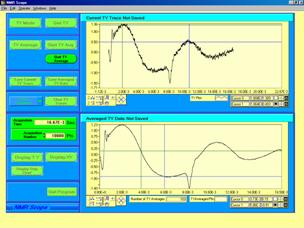
\includegraphics[width=\linewidth]{images/NMR38.jpg}} \\
        TY Mode
    \end{minipage}\hfill
    \begin{minipage}{0.49\linewidth}
        \centering
        \href{http://experimentationlab.berkeley.edu/sites/default/files/images/NMR39.jpg}{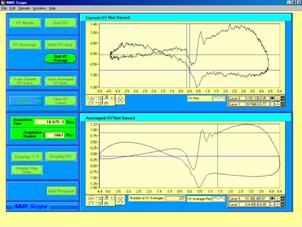
\includegraphics[width=\linewidth]{images/NMR39.jpg}} \\
        XY Mode
    \end{minipage}

    \item To stop the signal, press \textbf{Quit TY/XY Average}.
    
    \item To save the data press \textbf{Save Averaged TY/XY Data}.
    
    \item To clear the graphs press \textbf{Clear TY/XY Traces}.
\end{enumerate}

\emph{\textbf{Strip Chart Recording Function}} (used in the later part of the NMR experiment)

Instead of using the actual Strip Chart Recorder, we can use the NMR Scope2.0 program to accomplish the same results. Once all the equipment has been set up properly, the use of the program is simple.

\begin{enumerate}
    \item Set up the equipment as instructed in the section ``Taking Data,'' part E.

    \item Open the \textbf{NMR Scope2.0.vi} program.

    \item Press the button \textbf{Display Strip Chart}. You will see that you are only given one graph space in the top right corner.

    \item To start taking the data, press \textbf{Start Chart}. You will see something similar to the following graph:
    \begin{center}
        \href{http://experimentationlab.berkeley.edu/sites/default/files/images/NMR40.jpg}{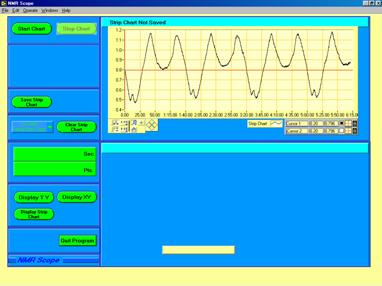
\includegraphics[width=0.5\linewidth]{images/NMR40.jpg}}
    \end{center}

    \item To stop the signal press \textbf{Stop Chart}

    \item To save the data press \textbf{Save Strip Chart}

    \item To clear the data press \textbf{Clear Strip Chart}
\end{enumerate}

This concludes the overview of the program. If you have any more questions, you can ask one of the staff members for help.

\section{REPORT}

Include the following data, analysis, and calculations.

\begin{enumerate}
    \item The Bloch Equations are the key to understanding this experiment:
    \begin{align}
        \label{eq:Bloch1}
        \frac{d}{dt} M_x &= \gamma (\vec{M} \times \vec{H})_x - \frac{M_x}{T_2} \\
        \label{eq:Bloch2}
        \frac{d}{dt} M_y &= \gamma (\vec{M} \times \vec{H})_y - \frac{M_y}{T_2} \\
        \label{eq:Bloch3}
        \frac{d}{dt} M_z &= \gamma (\vec{M} \times \vec{H})_z + \frac{(M_0 - M_z)}{T_1} 
    \end{align}

    \begin{enumerate}
        \item What is \textbf{M}? Is\textbf{ H} a magnetic field inherent in your sample, or is it an applied field? Derive equations \eqref{eq:Bloch1} to \eqref{eq:Bloch3} for the case of no damping (none of the $T_1$ or $T_2$ terms). Hint: consider the classical torque equation \textbf{N} = d\textbf{L}/dt.

        \item The equations you derived are applicable to a set of identical magnetic moments (spins), i.e., all the spins see the same magnetic field. The damping terms in \eqref{eq:Bloch1} to \eqref{eq:Bloch3} are added to take the different environment of each spin into account.

        \item In equations \eqref{eq:Bloch1} and \eqref{eq:Bloch2}, $T_2$ is often called a \emph{dephasing time}, the time required for (\textbf{M})x,y to decay to zero after the resonance condition is removed. What is getting out of phase? How can this arise from inhomogeneities in \textbf{H}?

        \item $T_1$ is the relaxation time for the z-component of \textbf{M} to come to an equilibrium value $M_0$ when the resonance condition (applied RF) is removed. (You can see this by setting \textbf{H} to zero in \eqref{eq:Bloch3}.) What determines this equilibrium value, and what is it? [Hint: look at the classical Boltzmann distribution.]

    \end{enumerate}

    \item What (very general) physical factor of your sample accounts for the magnitude of $T_1$? [Hint: $M_0$ is a thermal equilibrium magnetization.] More specifically, how might the addition of \emph{paramagnetic} ions Mn$^{++}$ affect $T_1$ (qualitatively)?

    \item Measure the magnetic field $H_0$ of the magnet as precisely as you can in Gauss (average value and standard deviation). Are paramagnetic corrections significant? Measure $H_0$ on several different days: does it vary? Why?

    \item Include best computer plot with calibrated H axes for proton signals in glycerin, showing the ``best wiggles.'' Estimate the magnetic field inhomogeneity from the damping rate of the wiggles.

    \item Computer plots with calibrated H axes for absorption and for dispersion NMR signals in H2O under slow passage and under non-adiabatic passage.

    \item Measure as precisely as you can the ratio of the magnetic moment of F$^{19}$ to H$^1$, with standard deviation. Show best scope photo of F$^{19}$ resonance.

    \item Record and show sequence of absorption lock-in trace from the computer for protons in the presence of M = 3, 1, 0.3, 0.1, 0.03 Molar Mn$^{++}$. Measure the line width (H in Gauss and plot (H vs. Molarity; explain this graph; what is the residual line width (in Gauss) due to field non-uniformity?

    \item From your best lock-in data for resonance in 1 Molar $Mn^{++M}$ in H2O, compute the expected S/N ratio for the deuteron resonance in a 1 Molar Mn$^{++}$ in D2O sample under two different assumptions:

    \begin{enumerate}
        \item The field $H_0$ is kept at 3800 G and the oscillator frequency is adjusted to f($H^2$).

        \item The oscillator frequency is kept at 16.1 MHz and the DC field is adjusted for resonance.

    \end{enumerate}

    \item Under condition 2 above, compute the S/N ratio expected for $O^{17}$ NMR resonance in naturally abundant water; compare to Ref.~\cite{Ames}, Fig. 4.

    \item Last day of the experiment please fill out the \href{\ExperimentEvaluation}{\textbf{Experiment Evaluation}}
\end{enumerate}

Revision 2013

Copyright (c) 2013 The Regents of the University California. All Rights Reserved

\begin{thebibliography}{}
\label{References}
    \bibitem{Abragam} A. Abragam, \emph{Principles of Nuclear Magnetism}, Oxford Press, 1961. This is the definitive reference.  Located in the Physics and Astronomy Library. \#QC762.A23

    \bibitem{Liboff} R. Liboff, \emph{Introduction Quantum Mechanics}, Holden Day, 1980. Sections 11.8 and 11.9 include a simple, direct derivation of NMR, along with a physical interpretation. While Liboff does not use the classical Bloch equations, he does give a good idea of what's going on. \#QC174.12.L54

    \bibitem{Walker} S. Walker and H. Straw, \emph{Spectroscopy Vol. 1}, Macmillian (1962, Ch. 5. (Available in 111 Lab, not to be taken out of the laboratory). \#QC451.W2 (Engineering Library)

    \bibitem{Bloch} Bloch, F., et al ``\href{http://prola.aps.org/abstract/PR/v70/i7-8/p474\_1}{\textbf{The Nuclear Induction Experiment}}''; Physical Review: Vol. 70, Oct 1946, pp. 474-485.(Note: Note check out CRC Table of Physical Constants for valves) \href{http://physics111.lib.berkeley.edu/Physics111/Reprints/NMR/04-The\_Nuclear\_Induction\_Experiment.pdf}{\textbf{Searchable Page}}

    \bibitem{Ames} Ames, D.P. ``\href{http://physics111.lib.berkeley.edu/Physics111/Reprints/NMR/05-Magnetic\_Resonance.pdf}{\textbf{Magnetic Resonance}}'': Chapter 9, pp. 8.112-8.127.

    \bibitem{Hahn} Hahn, E.L. ``\href{http://physics111.lib.berkeley.edu/Physics111/Reprints/NMR/06-Free\_Nuclear\_Induction.pdf}{\textbf{Free Nuclear Induction}}''; Physics Today, Nov. 1953, pp.4-9.

    \bibitem{Brewer} Brewer, Richard G. \& Hahn, Erwin L. ``\href{http://physics111.lib.berkeley.edu/Physics111/Reprints/NMR/07-Atomic\_Memory.pdf}{\textbf{Atomic Memory}}''; Scientific American: Vol. 251, No. 6, Dec. 1984, pp. 50-57.

    \bibitem{Lowe} Lowe, I.J., \& Whitson, D. ``\href{http://physics111.lib.berkeley.edu/Physics111/Reprints/NMR/08-Simple\_Pulsed\_NMR\_Spectrometer.pdf}{\textbf{Simple Pulsed Nuclear-Magnetic Resonance Spectrometer}}''; pp. 335-338.

    \bibitem{CohenTannoudji} Cohen-Tannoudji, ``\href{http://physics111.lib.berkeley.edu/Physics111/Reprints/NMR/09-Quantum\_Mechanics.pdf}{\textbf{Quantum Mechanics}}''; Vol. 1, 1977, Wiley. pp. 443-454.

    \bibitem{Jacobsohn} Jacobsohn, Boris A. and Wangsness, Roald ``\href{http://prola.aps.org/abstract/PR/v73/i9/p942\_1}{\textbf{Shapes of Nuclear Induction Signals}}''; Physical Review: Vol. 73, May, 1948, pp. 942-946. \href{http://physics111.lib.berkeley.edu/Physics111/Reprints/NMR/10-Shapes\_of\_Nuclear\_Induction\_Signals.pdf}{\textbf{Searchable Page}}

    \bibitem{Bloembergen} Bloembergen, N, Purcell, E. M., Pound, R.V. ``\href{http://prola.aps.org/abstract/PR/v73/i7/p679\_1}{\textbf{Relaxation Effects in Nuclear Magnetic Resonance Absorption}}''; Physical Review, Vol. 73, Apr, 1948, pp. 679-712. \href{http://physics111.lib.berkeley.edu/Physics111/Reprints/NMR/11-Relaxation\_Effects\_in\_NMR\_Absoprtion.pdf}{\textbf{Searchable Page}}

    \bibitem{NMRFrequencyTable} \href{http://experimentationlab.berkeley.edu/sites/default/files/images/NMR32.jpg}{\textbf{NMR Frequency Table}}
\end{thebibliography}

Other reprints and reference materials can be found on the \href{http://physics111.lib.berkeley.edu/Physics111/Reprints/NMR/NMR\_index.html}{\textbf{Physics 111 Library Site}}

\end{document}
